\documentclass[11pt]{article}
\usepackage[T1]{fontenc}
\usepackage{lmodern}
\usepackage{microtype}
\usepackage[utf8]{inputenc}
\usepackage{amsmath,amssymb,amsthm,mathtools}
\usepackage[a4paper,margin=24mm,headheight=14pt]{geometry}
\usepackage{graphicx,booktabs,longtable,array,xurl}
\usepackage[numbers,sort&compress]{natbib}
\usepackage{tikz,fancyhdr}
\pagestyle{fancy}
\fancyhf{}
\fancyhead[L]{\small Succinct Rabung certificates}
\fancyhead[R]{}\fancyfoot[C]{\thepage}
\renewcommand{\headrulewidth}{0.3pt}
\usepackage[colorlinks]{hyperref}
\hypersetup{allcolors=blue!40!black,
  pdftitle={Succinct Rabung certificates and recurrence-closed lower bounds for van der Waerden numbers},
  pdfauthor={Brice Pouly},
  pdfsubject={van der Waerden numbers},
  pdfkeywords={van der Waerden numbers, lower bounds, power residues, Rabung, GPU, certificates}}
\newtheorem{theorem}{Theorem}[section]
\newtheorem{proposition}[theorem]{Proposition}
\newtheorem{lemma}[theorem]{Lemma}\newtheorem{corollary}[theorem]{Corollary}
\newtheorem{conjecture}[theorem]{Conjecture}
\theoremstyle{definition}\newtheorem{definition}[theorem]{Definition}\newtheorem{remark}[theorem]{Remark}
\newcolumntype{P}[1]{>{\raggedright\arraybackslash}p{#1}}
\title{Succinct Rabung certificates and recurrence-closed\\
lower bounds for van der Waerden numbers}
\author{Brice Pouly\thanks{Prepared with artificial-intelligence assistance; see the declaration at the end.}}
\date{12 October 2026}
\hypersetup{pdfsubject={Publication edition v2.0; 12 October 2026}}
\begin{document}\maketitle
\begin{abstract}
Rabung's power-residue construction describes a large progression-free
colouring by a prime, a colour count and a target length. We give six
additional primitive certificates, checked by full ordinary CPU scans,
which yield fourteen direct lower bounds. In colour-first notation, these
include $W(3,17)>33\,166\,190\,897$, $W(3,18)>100\,289\,348\,022$,
$W(3,19)>259\,446\,988\,783$ and $W(3,20)>326\,368\,775\,450$.
The larger ternary primes lie outside the complete census below $2^{32}$.
We prove the equivalence of the run and boundary tests with Rabung's
criterion and separate pointwise verification from discovery. A finite
closure of explicitly identified earlier constructions places the new
bounds in context: direct ternary certificates win through length $23$;
Berlekamp and binary recurrence inputs win thereafter. Exact-modulus
cyclic witnesses also give six-colour product bounds. The previously
published thirteen-claim evidence and its closed empirical analyses are
retained separately. Comparisons refer to the stated source catalogue,
without an exhaustive global priority or optimality claim.
\end{abstract}
\noindent\textbf{Keywords.} Van der Waerden numbers; power-residue colourings;
Rabung certificates; computational Ramsey theory.
\clearpage
\setcounter{tocdepth}{1}
\tableofcontents
\bigskip
% ============ STRUCTURE ============
\section{Introduction}\label{s:intro}

A lower bound for a van der Waerden number is witnessed by a colouring that
avoids long monochromatic arithmetic progressions. At the sizes considered
here, such a colouring contains tens of billions of positions. Its description,
however, need not be comparably large. In Rabung's power-residue construction,
a triple of integers $(p,r,k)$ determines the finite conditions from which the
colouring and its lower bound follow. The computational problem is to find a
useful triple; the mathematical problem is to verify those conditions and to
place the bound among the consequences of earlier constructions.

For integers $r\ge2$ and $k\ge3$, let $W(r,k)$ be the least $N$ such that
every $r$-colouring of $\{1,\dots,N\}$ contains a monochromatic arithmetic
progression of length $k$. We put colours first. Monroe~\cite{Monroe2026}
uses the reverse convention $W(k,r)$; Fox and Hunter~\cite{FoxHunter2026}
write $w(k;r)$.

\subsection{Current results and their evidence}
Six additional primitive certificates give fourteen direct inequalities.
The four leading ternary bounds are
\[
\begin{aligned}
 W(3,17)&>33\,166\,190\,897, & W(3,18)&>100\,289\,348\,022,\\
 W(3,19)&>259\,446\,988\,783, & W(3,20)&>326\,368\,775\,450.
\end{aligned}
\]
Theorem~\ref{thm:update} gives the certificates and their mathematical
implications. In the extended admitted comparison, the direct ternary
rows win through length $23$; new binary inputs give stronger recurrence
consequences at $27$ and $28$, and exact cyclic witnesses yield six-colour
products. The larger ternary primes are pointwise constructions outside
the complete census below $2^{32}$.

The published edition~\cite{publishededition} and its thirteen-claim
evidence are retained separately. New pointwise executions and a separate
recurrence graph are not retroactively inserted into that evidence.
The new inequalities use full ordinary CPU rechecks. Complete search
coverage, scanner performance and the algebraic classification of a census
have separate evidence requirements; neither a timing measurement nor a
proposed law of maxima enters the lower-bound proof.


\subsection{Results of the published edition}

The published edition obtained three primitive three-colour Rabung certificates, at lengths
$17$, $18$ and $19$. They give nine direct inequalities for $17\le k\le25$;
the final six follow from the length-19 certificate by a fixed-prime
monotonicity lemma. In particular,
\[
 W(3,17)>31\,385\,622\,833,
\]
using $p=1\,961\,601\,427$. This is a factor $2.02$ above the earlier
$15\,509\,557\,937$ listed by Monroe. The five inequalities for
$17\le k\le21$ improve the prior comparators identified in the source review
updated on 26~September~2026; Table~\ref{tab:priority} gives their values.

A new direct certificate need not give a better general bound. For
$22\le k\le25$, our certificates improve the Rabung rows located in the
review, but stronger bounds already follow from other constructions. A
stronger published statement of Landman and Robertson has an unresolved
proof status in our audit. We display its consequences separately and include
it among prior comparators: the five improvements at lengths $17$--$21$
remain, whereas it dominates that edition's admitted table at lengths
$24$--$28$. Section~\ref{s:update} gives the current comparison.
This is a comparison with a dated, explicit corpus, not an assertion of
exhaustive global priority.

We also recheck four two-colour certificates from the archived second phase of
Monroe's distributed project~\cite{MonroePhase2Archive}, retaining the credit
of that project and its volunteers. Together with the nine three-colour rows,
they form the thirteen inequalities of Theorem~\ref{thm:certified-rabung}.
Only seven triples are primitive; the archived rechecks deliberately retain
the redundant consequences.

\subsection{From a short certificate to a finite comparison}

Multiplication by a nonzero residue permutes the colour classes of a
power-residue colouring. After such a dilation, an arithmetic progression
becomes a consecutive string. Rabung's theorem reduces the large-colouring
problem to a run-length test and a condition at the multiples of
$p$~\cite{rabung1979}. A qualifying prime gives $W(r,k)>(k-1)p+1$.
We prove the equivalence of the implemented boundary test with the published
criterion and provide a stand-alone CPU checker whose source and arithmetic
are separate from the GPU search. The small example in
Section~\ref{ss:criterion} illustrates the reduction before the proof.

\begin{figure}[htbp]
\centering
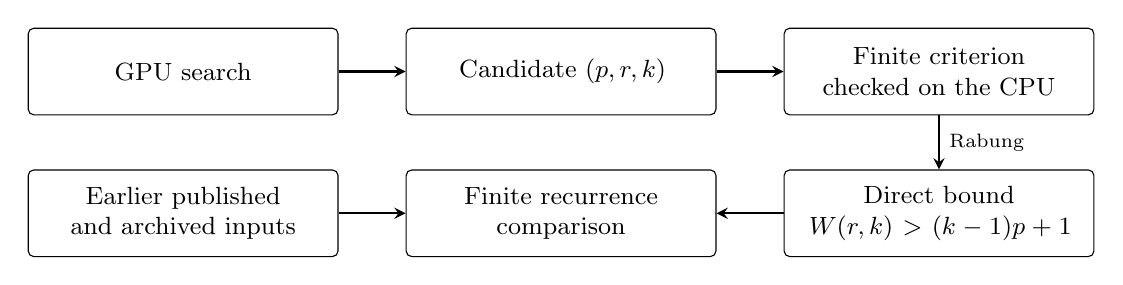
\begin{tikzpicture}[>=stealth,box/.style={draw,rounded corners=2pt,
  align=center,font=\small,minimum height=11mm,text width=3.7cm},
  edge/.style={->,thick}]
\node[box] (search) at (0,0) {GPU search};
\node[box] (triple) at (4.8,0) {Candidate $(p,r,k)$};
\node[box] (check) at (9.6,0) {Finite criterion\\checked on the CPU};
\node[box] (prior) at (0,-1.8) {Earlier published\\and archived inputs};
\node[box] (closure) at (4.8,-1.8) {Finite recurrence\\comparison};
\node[box] (bound) at (9.6,-1.8) {Direct bound\\$W(r,k)>(k-1)p+1$};
\draw[edge] (search)--(triple);
\draw[edge] (triple)--(check);
\draw[edge] (check)--node[right,font=\scriptsize]{Rabung}(bound);
\draw[edge] (bound)--(closure);
\draw[edge] (prior)--(closure);
\end{tikzpicture}
\caption{The two steps after discovery. The candidate can be checked without
replaying the search, and its bound is compared with consequences of earlier
inputs. Campaign coverage and the empirical intensity analysis are separate
from these pointwise implications.}
\label{fig:evidence-flow}
\end{figure}



Earlier bounds must then be compared under known recurrences. For example,
Blankenship, Cummings and Taranchuk~\cite[Theorem~2.1]{bct2018} prove
\begin{equation}\label{eq:bct-intro}
 W(r,k)>q\left(W\!\left(r-\left\lceil r/q\right\rceil,k\right)-1\right)
\end{equation}
for a prime $q\le k$. For three colours, an earlier strict bound
$W(2,k)>B$ gives $W(3,k)>q_kB$, where $q_k$ is the largest prime at most
$k$. This explains why a larger Rabung prime need not yield the strongest
general bound. Our finite comparison also includes length monotonicity and
the registered Xu operation~\cite{xu2013,Monroe2026}, with exact integers
and a provenance path for every retained value. No winning three-colour row
depends on Xu.

\subsection{Relation to earlier work}

Computational power-residue constructions and cyclic-zipper extensions have
been developed by Herwig, Heule, van Lambalgen and van Maaren~\cite{herwig2007},
Rabung and Lotts~\cite{rabunglotts2012}, Liang, Xu, Shao and
Xiu~\cite{liang2012}, and Monroe~\cite{Monroe2016v1,Monroe2017v4,Monroe2026}.
Publishing a prime together with checking code has antecedents in this
literature. The published edition contributed three new primitive certificates, their
separate verification, and their explicit comparison with consequences of
the identified prior inputs. This revision adds the six primitive certificates
of Section~\ref{s:update}. Certification is not presented as a new principle.

Berlekamp's construction supplies a stronger admitted bound at length $24$,
inherited at length $25$~\cite{Berlekamp1968}. The stronger
Landman--Robertson statement requires the separate treatment just
described~\cite{LandmanRobertson2004,LandmanRobertson2014,Johannson2007}.
The recent superexponential three-colour result of Fox and
Hunter~\cite{FoxHunter2026} and the asymptotic two-colour bound
$w(k)\ge(1-o(1))k2^{k-1}$ of Campos, Fox and
Schildkraut~\cite{CamposFoxSchildkraut2026} address different asymptotic
questions. In the version-pinned sources examined, neither supplies a
stronger explicit finite entry for our window.
Gasarch and Haeupler's explicit family
$W(3,k)\ge3^{k-1}/(ek)$~\cite[Note~1.7(2)]{GasarchHaeupler2011} is retained
in the registry and is dominated there. Kozik and
Shabanov~\cite[Theorem~2 of the arXiv version]{KozikShabanov2014} give
$W(r,k)\ge\beta r^{k-1}$ for an absolute $\beta>0$; no finite improvement
from that theorem is asserted here. Hunter's exponential improvement begins
at five colours~\cite{Hunter2025} and does not change the three-colour table.

\subsection{Reading guide and evidence boundary}

Section~\ref{s:update} gives the revised numerical results;
Section~\ref{s:bounds} retains the published comparison and claim identities.
Section~\ref{s:method} explains the construction, proves the boundary-test
equivalence and describes the checker. Section~\ref{s:campaign} explains
the discovery and verification protocol. The search covered
$[9.7\times10^8,2\times10^9)$ in $515$ chunks; its coverage evidence has a
separate role from the validity of any one certificate.

A reader interested in the inequalities can read the results and the
criterion proof first. The witness is short, but a complete recheck still
visits a linear number of residues and evaluates their colours; checking the
identities of the retained archive is a separate, much lighter operation. The source catalogue, campaign audit and execution
identities remain available in the appendices and accompanying package.
Appendices~\ref{s:prereg}--\ref{s:densitydiagnostics} compare three fixed
search-intensity forecasts on one run-valid $(3,17)$ trajectory. That empirical
comparison neither proves a density law nor enters the lower-bound proof.
No independently administered external replication has been performed; the
preserved local computations and their limits are stated throughout.


\section{Current certificate addendum and its closure}\label{s:update}

The additional certificates were recorded on 9 October 2026. It imports the admitted inputs of
the published edition and adds pointwise certificates from the complete
atlas and from subsequent targeted searches. The latter searches are not
claimed to enumerate a new interval exhaustively. The finite comparison
now permits up to six colours, while keeping lengths $12$ through $28$.
The original four-colour closure and thirteen-claim execution gate remain
unchanged as historical artifacts.

\subsection{Six primitive certificates}

For a character colouring of the nonzero residues, $M$ is the longest
ordinary consecutive run and $L$ the initial run starting at $1$.
The least construction threshold is
\[
 K=\max(M+1,2L+2)\quad\text{if }\chi(-1)=1,
 \qquad K=\max(M+1,L+2)\quad\text{otherwise}.
\]
Section~\ref{s:bstar} proves why these thresholds encode Rabung's
boundary condition. They are thresholds for construction, not additional
run lengths.

% Generated from retained full CPU executions.
\begin{table}[htbp]\centering\small
\begin{tabular}{rrrrrr}\toprule $r$ & minimum $k$ & $p$ & $M$ & $L$ & $K$\\\midrule
3 & 17 & $2\,072\,886\,931$ & 16 & 1 & 17\\
3 & 18 & $5\,899\,373\,413$ & 17 & 2 & 18\\
3 & 19 & $14\,413\,721\,599$ & 18 & 2 & 19\\
3 & 20 & $17\,177\,303\,971$ & 19 & 1 & 20\\
2 & 27 & $4\,195\,501\,393$ & 26 & 4 & 27\\
2 & 28 & $4\,294\,720\,151$ & 27 & 6 & 28\\
\bottomrule\end{tabular}
\caption{Six primitive certificates of the addendum, rechecked by full ordinary CPU scans. Four ternary and two binary triples give fourteen direct inequalities in the reported window.}\label{tab:updated-primitive}
\end{table}


\begin{theorem}[Current pointwise bounds]\label{thm:update}
Each triple in Table~\ref{tab:updated-primitive} satisfies Rabung's
conditions at its displayed minimum length. Consequently,
\begin{align*}
 W(3,17)&>33\,166\,190\,897, &
 W(3,18)&>100\,289\,348\,022,\\
 W(3,19)&>259\,446\,988\,783, &
 W(3,20)&>326\,368\,775\,450,\\
 W(2,27)&>109\,083\,036\,219, &
 W(2,28)&>115\,957\,444\,078.
\end{align*}
The length-$20$ ternary certificate also gives
$W(3,k)>(k-1)17\,177\,303\,971+1$ for $21\le k\le28$.
These are fourteen direct rows from six primitive certificates.
\end{theorem}

\begin{proof}[Computational proof and mathematical implication]
The retained complete CPU executions re-establish primality, the full
factorisation tests for a primitive root, and the character table by a
multiplicative walk through every nonzero residue. The ordinary scan then
visits all $p-1$ positions, determines $M$ and $L$, and explicitly evaluates
the boundary condition $B^*$. Every record reports acceptance and the
values in Table~\ref{tab:updated-primitive}. In particular $M<k$ and
$K\le k$. Rabung's theorem and Proposition~\ref{p:bstar} imply
$W(r,k)>(k-1)p+1$. Lemma~\ref{lem:k-monotone} supplies the eight further
lengths at the fixed prime. The source and execution identities, and the
distinction between a full scan and the lightweight record audit, are
specified below.
\end{proof}

The three smaller primitive primes belong to the atlas domain $p<2^{32}$.
The three larger ternary primes in the table do not; the two descriptions
overlap in neither coverage nor any claim of maximality beyond that
domain. Nine full rechecks were performed in total. Six bind the atlas
targets at $(3,17)$--$(3,20)$, $(2,27)$ and $(2,28)$ to their catalogue
entries; three check the stronger ternary primes used here. At lengths
$18$--$20$ the atlas entries are therefore useful verified certificates,
but the larger pointwise certificates give the current direct rows.
The length-$17$ improvement over the published edition is approximately
$5.67\%$. No literature-wide priority update is inferred from that
comparison.

\subsection{Updated admitted comparison}

% Generated by scripts/verify_bounds_update.py --generate.
\begin{table}[htbp]\centering\small\setlength{\tabcolsep}{4pt}
\begin{tabular}{rrrrl}\toprule $k$ & direct $p$ & direct strict bound & closed strict bound & method\\\midrule
17 & $2\,072\,886\,931$ & $33\,166\,190\,897$ & $33\,166\,190\,897$ & direct Rabung\\
18 & $5\,899\,373\,413$ & $100\,289\,348\,022$ & $100\,289\,348\,022$ & direct Rabung\\
19 & $14\,413\,721\,599$ & $259\,446\,988\,783$ & $259\,446\,988\,783$ & direct Rabung\\
20 & $17\,177\,303\,971$ & $326\,368\,775\,450$ & $326\,368\,775\,450$ & direct Rabung\\
21 & $17\,177\,303\,971$ & $343\,546\,079\,421$ & $343\,546\,079\,421$ & direct Rabung\\
22 & $17\,177\,303\,971$ & $360\,723\,383\,392$ & $360\,723\,383\,392$ & direct Rabung\\
23 & $17\,177\,303\,971$ & $377\,900\,687\,363$ & $377\,900\,687\,363$ & direct Rabung\\
24 & $17\,177\,303\,971$ & $395\,077\,991\,334$ & $1\,082\,646\,556\,499$ & Berlekamp\\
25 & $17\,177\,303\,971$ & $412\,255\,295\,305$ & $1\,082\,646\,556\,499$ & Berlekamp + mono.\\
26 & $17\,177\,303\,971$ & $429\,432\,599\,276$ & $1\,221\,912\,599\,848$ & BCT\\
27 & $17\,177\,303\,971$ & $446\,609\,903\,247$ & $2\,508\,909\,833\,037$ & BCT\\
28 & $17\,177\,303\,971$ & $463\,787\,207\,218$ & $2\,667\,021\,213\,794$ & BCT\\
\bottomrule\end{tabular}
\caption{Updated three-colour bounds, all in the strict convention $W(3,k)>B$. The direct rows use four primitive ternary certificates. Closed values include the two new binary inputs and the admitted published seeds. The unresolved Landman--Robertson statement remains a separate comparator; no unrestricted optimality is asserted.}\label{tab:updated-closed}
\end{table}


Table~\ref{tab:updated-closed} is generated by the original closure
program with a separate merged input registry. It admits the published
seeds and the new certificates, applies the same exact-integer operators,
and retains a provenance graph. The direct certificates now dominate the
admitted three-colour comparison for $17\le k\le23$. Berlekamp's
specialization still wins at $24$ and its monotone consequence at $25$;
the BCT operation wins at $26$--$28$. In particular the new binary inputs
give
\begin{align*}
 W(3,27)&>23\times109\,083\,036\,219
            =2\,508\,909\,833\,037,\\
 W(3,28)&>23\times115\,957\,444\,078
            =2\,667\,021\,213\,794.
\end{align*}
The unresolved Landman--Robertson statement keeps the status explained
in Section~\ref{s:bounds}. Its separately displayed strict comparator
$2\,165\,293\,112\,998$ exceeds the admitted revised bounds at
$24$--$26$, but no longer at $27$ or $28$. It is not silently promoted
to an admitted proof input. A winning value in this finite graph is not
an unrestricted best possible bound.

\subsection{Exact-modulus six-colour products}

The new ternary certificates also give cyclic witnesses at their actual
prime moduli. Their least prime divisors are the moduli themselves and
exceed $k$, as required by the exact-witness product
\eqref{eq:xu}. With the admitted two-colour inputs of
Liang et al.~\cite{liang2012}, this gives
\begin{align*}
 W(6,18)&>5\,899\,373\,413\times91\,079\,252
       =537\,310\,517\,724\,727\,076,\\
 W(6,19)&>14\,413\,721\,599\times250\,546\,915
       =3\,611\,313\,480\,298\,317\,085,\\
 W(6,20)&>17\,177\,303\,971\times526\,317\,462
       =9\,040\,715\,030\,019\,241\,602.
\end{align*}
The graph records each cyclic parent and ordinary parent separately.
The product uses the modulus $p$, rather than the much larger ordinary
Rabung construction length. All displayed values are strict integer
bounds $W>B$; the equivalent weak form is $W\ge B+1$.

\subsection{Separate-source rechecks and reproduction scope}

The addendum provides two ordinary CPU checkers. Neither imports the GPU
scanner, its arithmetic, sparse cover, or reduction code. The byte-table
checker handles $p<2^{32}$ and orders $2$ through $9$ using exact
64-bit products. The two-bit checker handles orders $2$ and $3$,
$p<2^{35}$, target lengths at most $256$, and an explicit product-capacity
guard. It uses exact 128-bit products for powering and checked 64-bit
products for the multiplicative walk. These are CPU domains and do not
extend the GPU worker's proved domain. At the largest prime, the packed
table occupies approximately $4.3$ GB.

The records in \path{reproducibility/bounds_update/results/} contain the
source and binary hashes, compiler, command, literal output and exit status
of all nine full scans. Their arithmetic checks and ordinary scan use no
reflection or sparse-cover assumption. Sample powering and reflection
checks are additional diagnostics; the global upper bound on $M$ comes
from visiting the entire period, not from those samples. The computations
are author-controlled, with separate source from the GPU discovery path;
they are not independently administered external replications.

The bounded command \path{scripts/verify_bounds_update.py} checks retained
identities, primes and root orders, literal local powers, catalogue binding,
the unchanged published closure, and the regenerated current graph. It
does not rescan the billion-position words. Small controls compare both
new checkers with direct power colours and literal arithmetic progressions,
and exercise refusal cases. Repeating a large check requires rebuilding
the relevant checker and running it on $p\ r\ k$; this is a separate
complete calculation. Neither a new GPU campaign nor any probability law
is required for these pointwise consequences.


\section{Results of the published edition (v1.0)}\label{s:bounds}
The tables and execution counts in this section retain the edition
published as v1.0.0~\cite{publishededition}, with its source review cut off
on 26 September 2026. They are historical comparison tables.
Section~\ref{s:update} gives the current addendum and its updated closure.
Paths for the original claim gate, campaign and holdout refer to that
edition's artifact; selected original registries are copied unchanged in
\path{reproducibility/bounds_update/published_v1_0/}.


The computation gives the thirteen direct inequalities stated below: nine
at three colours and four re-verifications of earlier two-colour certificates.
Their supporting evidence consists of archived executions bound to exact
source code, binaries and raw output. Checking the archive and rebuilding this
paper requires no repetition of the GPU campaign.

%
  \begin{theorem}[Certified Rabung bounds]\label{thm:certified-rabung}
  For every triple $(p,r,k)$ in Table~\ref{tab:validated-claims}, $p$ is
  prime, $p\equiv1\pmod r$, $p>k$, and the power-residue colouring satisfies
  conditions $(a)\wedge(B^{*})$. Consequently
  \[
    W(r,k)>(k-1)p+1.
  \]
  In particular, all thirteen direct inequalities registered in
  \texttt{audit/claims.json} hold.
  \end{theorem}
  \begin{proof}
  At each listed prime, the full scan finds $M<k$ and checks the boundary
  strings $(B^{*})$. It also checks primality, $p\equiv1\pmod r$ and
  $p>k$. Proposition~\ref{p:bstar} identifies
  $(B^{*})$ with Rabung's boundary criterion. Rabung's theorem therefore
  constructs a progression-free colouring of $(k-1)p+1$ positions.
  The stand-alone checker and its retained execution results are described in
  Section~\ref{ss:certificates} and Appendix~\ref{s:certificate-evidence};
  The retained file identities are checked before building the table.
  \end{proof}
  The full execution-identity table is provided in Appendix~\ref{s:certificate-evidence}.


\subsection{Three colours: direct and recurrence-closed bounds}\label{ss:r3}

The nine three-colour rows involve only three distinct primes. By
Lemma~\ref{lem:k-monotone}, the certificate
$(1\,999\,999\,927,3,19)$ implies all six rows with the same prime and
$20\le k\le25$. Thus only seven triples in the thirteen-row theorem are
mathematically primitive: three at three colours and the four two-colour
triples below. The evidence package nevertheless re-evaluates the complete
criterion at all thirteen registered triples as deliberate audit redundancy;
the six repeated checks are neither mathematically necessary nor counted as
independent implementation paths.

The headline value
\[
  W(3,17)>31\,385\,622\,833
\]
comes from $p=1\,961\,601\,427$ and improves Monroe's published
$15\,509\,557\,937$ by a factor $2.02$~\cite{Monroe2026}.  A direct
certificate is not automatically a general record: a published bound in
another colour column may imply a stronger result through a recurrence.

Table~\ref{tab:priority} states the five improvements against the earlier
comparators identified in our review. For this comparison the new three-colour
claims are removed from the finite closure, and the published
Landman--Robertson statement is included as a conservative comparator even
though its proof was not verified here. Thus the comparison does not obtain
an artificial gain by discarding that statement.

% Generated by tools/publication_comparison.py; do not edit.
\begin{table}[htbp]
\centering\small
\begin{tabular}{@{}c r r l@{}}
\toprule
$k$ & new strict bound & prior comparator & comparator source \\
\midrule
17 & $31\,385\,622\,833$ & $15\,509\,557\,937$ & Monroe tally \\
18 & $33\,999\,912\,468$ & $16\,479\,723\,552$ & Monroe tally \\
19 & $35\,999\,998\,687$ & $17\,449\,137\,523$ & Monroe tally \\
20 & $37\,999\,998\,614$ & $22\,082\,967\,854$ & Landman--Robertson$^{*}$ \\
21 & $39\,999\,998\,541$ & $26\,783\,744\,079$ & BCT from two colours \\
\bottomrule
\end{tabular}
\caption{Historical comparison retained from the published edition. The five improvements over prior comparators identified through
26 September 2026. Every numerical entry $B$ uses the strict convention
$W(3,k)>B$. $^{*}$The published Landman--Robertson statement is included
for a conservative comparison; its proof was not verified in our review.
The finite prior closure excludes the new three-colour claims.}
\label{tab:priority}
\end{table}



Let $q_k$ denote the largest prime not exceeding $k$.  From
Blankenship--Cummings--Taranchuk~\cite[Theorem~2.1]{bct2018},
\[
  W(3,k)>q_k\bigl(W(2,k)-1\bigr).
\]
Their theorem permits every prime $q\le k$. For three colours, $q=2$ reduces
to the one-colour case, while every $q\ge3$ uses the same two-colour input;
choosing the largest such prime therefore loses no BCT consequence for the
three-colour outputs considered here.
If the registered input is the strict integer bound $W(2,k)>B$, then
$W(2,k)-1\ge B$, and the generated consequence is exactly
\begin{equation}\label{eq:bct-r3}
  W(3,k)>q_k B,
\end{equation}
with no off-by-one ambiguity.

For example, the published input $W(2,22)>2\,582\,037\,634$ gives
\[
 W(3,22)>19\times2\,582\,037\,634=49\,058\,715\,046,
\]
which exceeds the direct value $41\,999\,998\,468$ retained from the
published edition. In that comparison, length $22$ is the first at which
a direct row loses to a recurrence consequence. The current frontier is
length $24$, as Table~\ref{tab:updated-closed} shows.

We use Xu's concatenation in its \emph{exact-witness} form
\cite{xu2013,Monroe2026}. Let $k\ge3$, $s\ge2$, $t\ge1$, and suppose an
$s$-colouring of $\mathbb Z/R\mathbb Z$ contains no nonzero-step $k$-term
arithmetic progression. Require $R\ge5$ and that the least prime divisor
of $R$ exceed $k$; the terms of every such progression are then distinct.
If $W(t,k)>B$, concatenation gives
\begin{equation}\label{eq:xu}
  W(st,k)>RB.
\end{equation}
Indeed, write $x=Rq+a$ for $0\le x<RB$, with $0\le a<R$, and colour $x$
by the pair consisting of the cyclic colour of $a$ and a progression-free
$t$-colouring of $q\in\{0,\ldots,B-1\}$. A monochromatic progression whose
step is not divisible by $R$ contradicts the cyclic colouring; if its step
is divisible by $R$, its block indices contradict the ordinary colouring.
Thus the product bound uses a colouring at the specific modulus $R$.

A lower bound for a cyclic threshold alone would not supply this witness.
The registry's \texttt{ring\_seeds} therefore records exact moduli, together
with their source attribution or Rabung claim identity. For a Rabung input,
conditions $(a)\wedge(B^{*})$ also give the cyclic colouring at modulus $p$:
a nonzero step dilates to consecutive residues, and windows meeting zero
are excluded by $(B^{*})$, whatever colour is assigned to zero.
The published witness inputs retain their cited provenance; they are not
new large computations of this work. The original full text of Xu was not
obtained in the latest review; its use in the preceding literature was read
in Monroe's account. The exact-witness product argument above makes the
operation used here explicit. No winning three-colour row depends on Xu.

The baseline program iterates elementary length monotonicity, the registered
BCT specialization and \eqref{eq:xu} to a fixed point. Its closure state covers
$12\le k\le28$ and at most four colours; the reported comparison window remains
$17\le k\le28$. Published direct and Berlekamp seeds are loaded from $k=12$
so earlier monotone consequences are not truncated. At each step it retains exact integer
bounds and a full provenance path. Candidates are compared first by bound;
numerical ties use the deterministic order direct Rabung, published or archived
seed, length monotonicity, BCT, Xu, one-colour exact, and finally the
hash-derived node identifier. These tie-breaks affect provenance only. Since
all three operators are monotone in their input bounds, a dominated parent
cannot improve a descendant. Iteration stops when no winning node changes.

The seed registry and its dated source catalogue are detailed in
Appendix~\ref{s:source-catalogue}. Published and archived predecessors are
loaded from length $12$, so consequences entering the reported window from
earlier lengths are retained. Throughout this paper, an \emph{admitted bound}
means a consequence of those explicitly registered inputs and operations.
The separately displayed Landman--Robertson statement has a different status.

Berlekamp writes $W(K,t)$ for $K$ colours and progressions of length $t+1$.
Specializing his Theorem~1 to $K=3,t=23$ gives
\begin{equation}\label{eq:berlekamp-24}
  W(3,24)>\frac{23(3^{23}-1)}{2}
           =1\,082\,646\,556\,499,
\end{equation}
after checking the theorem's divisor conditions~\cite{Berlekamp1968}. Length
monotonicity gives the same strict bound for $W(3,25)$. The registry also
contains the sixteen directly dominated specializations, so this winning case is not an
isolated post hoc insertion.

Landman and Robertson state, without an accompanying proof, that for primes
$p\ge5$ and $q$,
\[
  w(p+1;q)\ge p(q^p-1)+1
\]
in their first and second editions~\cite[Theorem~2.19, p.~38]{LandmanRobertson2004}
\cite[Theorem~2.21, p.~43]{LandmanRobertson2014}.
For $q=3$, its specializations at $p=19$ and $p=23$ give respectively
\[
 W(3,20)>22\,082\,967\,854,
 \qquad W(3,24)>2\,165\,293\,112\,998.
\]
In the comparison retained from the published edition, the latter would
dominate through $k=28$ by length monotonicity. The updated admitted values
exceed it at $27$ and $28$ (Section~\ref{s:update}). Berlekamp's primary construction proves the general factor
$1/(q-1)$, with its stronger extension confined to $q=2$, and Johannson's
detailed reconstruction reports that the proposed general adaptation could
not be confirmed~\cite[pp.~88--90]{Johannson2007}.
This does not disprove the textbook statement. It is excluded from the numerical registry
of admitted constructions and certificates, but retained as a
published statement with unresolved proof status in our audit.
Table~\ref{tab:unresolved} makes its numerical effect explicit. In particular,
the admitted values for $24\le k\le28$ must not be described without this
qualification as the best published bounds. The $k=20$ specialization is
already included in Table~\ref{tab:priority} and does not remove that improvement.

% Generated by tools/publication_comparison.py; do not edit.
\begin{table}[htbp]
\centering\small
\begin{tabular}{@{}c r r@{}}
\toprule
$k$ & best admitted consequence & published unresolved statement \\
\midrule
20 & $37\,999\,998\,614$ & $22\,082\,967\,854$ \\
24 & $1\,082\,646\,556\,499$ & $2\,165\,293\,112\,998$ \\
25 & $1\,082\,646\,556\,499$ & $2\,165\,293\,112\,998$ \\
26 & $1\,221\,912\,599\,848$ & $2\,165\,293\,112\,998$ \\
27 & $2\,068\,976\,009\,617$ & $2\,165\,293\,112\,998$ \\
28 & $2\,159\,051\,058\,266$ & $2\,165\,293\,112\,998$ \\
\bottomrule
\end{tabular}
\caption{Historical comparison retained from the published edition; the current comparison is in Section~\ref{s:update}. The middle column uses the checked
seed registry, including this work. The last column records the numerical
consequences of the stronger published Landman--Robertson statement and
length monotonicity; these are not certified by this paper.}
\label{tab:unresolved}
\end{table}



The arXiv version history dates Monroe's earlier
$W(3,17)>15\,509\,557\,937$ and prime $969\,347\,371$ to version~4 of
6~November~2017; versions~1--3 do not contain them~\cite{Monroe2017v4}.
Exact-number, prime, publisher, preprint, citation-chain, repository and web
archive searches were performed. No earlier public source was located for the
three primitive direct triples used here at $k=17,18,19$ in the review updated
on 26~September~2026. This bounded search result does not establish global priority. We therefore describe those certificates as new to
the audited corpus rather than assert an unqualified first discovery. The
search methods, version pins, admitted and excluded findings, and exact cutoff
are machine-readable in \texttt{publication/bibliography-audit.json}.

% Generated by tools/close_baselines.py; do not edit by hand.
\begin{table}[ht]
\centering\footnotesize
\begin{tabular}{c r r r l}
\toprule
$k$ & direct $p$ & direct bound & winning admitted bound & method \\
\midrule
17 & $1\,961\,601\,427$ & $31\,385\,622\,833$ & $31\,385\,622\,833$ & direct Rabung \\
18 & $1\,999\,994\,851$ & $33\,999\,912\,468$ & $33\,999\,912\,468$ & direct Rabung \\
19 & $1\,999\,999\,927$ & $35\,999\,998\,687$ & $35\,999\,998\,687$ & direct Rabung \\
20 & $1\,999\,999\,927$ & $37\,999\,998\,614$ & $37\,999\,998\,614$ & direct Rabung \\
21 & $1\,999\,999\,927$ & $39\,999\,998\,541$ & $39\,999\,998\,541$ & direct Rabung \\
22 & $1\,999\,999\,927$ & $41\,999\,998\,468$ & $49\,058\,715\,046$ & BCT, $q=19$ (published $W(2,k)$) \\
23 & $1\,999\,999\,927$ & $43\,999\,998\,395$ & $142\,741\,265\,701$ & BCT, $q=23$ (published $W(2,k)$) \\
24 & $1\,999\,999\,927$ & $45\,999\,998\,322$ & $1\,082\,646\,556\,499$ & Berlekamp (1968) \\
25 & $1\,999\,999\,927$ & $47\,999\,998\,249$ & $1\,082\,646\,556\,499$ & Berlekamp + length monotonicity \\
26 & -- & -- & $1\,221\,912\,599\,848$ & BCT, $q=23$ (archived input) \\
27 & -- & -- & $2\,068\,976\,009\,617$ & BCT, $q=23$ (archived input) \\
28 & -- & -- & $2\,159\,051\,058\,266$ & BCT, $q=23$ (archived input) \\
\bottomrule
\end{tabular}
\caption{Historical comparison retained from the published edition; Section~\ref{s:update} gives the extended comparison. Direct three-colour Rabung certificates and the winning lower bounds
obtained after closing the audited, admitted baselines under length monotonicity and the published
Blankenship--Cummings--Taranchuk and Xu recurrences.  A dash means that the
GPU campaign made no direct three-colour claim for that length.  For
$k=22,23,24,25$ the direct certificates are the strongest direct Rabung bounds
located in the audited corpus but do not win the admitted comparison. Every entry is generated with a
machine-readable provenance path in \texttt{audit/generated/bounds\_closure.json}.
The stronger published Landman--Robertson statement is listed separately in
Table~\ref{tab:unresolved}; this is not an unqualified table of best published bounds.}
\label{tab:r3}
\end{table}



%
\begin{corollary}[Historical recurrence-closed consequences]\label{cor:closed-bounds}
Within the published edition's frozen seed set and finite scope, closing under the
length-monotonicity, Blankenship--Cummings--Taranchuk and Xu operations gives
the winning strict bounds in Table~\ref{tab:r3}. In particular, the certified
direct rows win for $17\le k\le21$, while for $22\le k\le25$ they are dominated
by the displayed admitted consequences.
\end{corollary}


In the comparison retained from the published edition, the certified rows
for $17\le k\le21$ give the strongest bounds located
in the registered, recurrence-closed source corpus. For $22\le k\le25$ the
direct rows improve the direct Rabung family but do not win the admitted
comparison. BCT consequences of published two-colour values win at $k=22,23$;
Berlekamp wins at $k=24,25$. No winning three-colour row in this finite scope
uses Xu's recurrence; it is retained because the comparison claim includes all
registered operations.

\subsection{Archived two-colour inputs and recurrence consequences}\label{ss:r2}

After the scan, we located a table from a second, unpublished phase of Daniel
Monroe's Vdwnumbers.org BOINC project (2021, two colours only)~\cite{MonroePhase2Archive}.
The earliest public evidence located in our audit attributes the four values
to that project and its volunteer contributors. A later author-owned project
page reports retrospectively that this phase pushed the checked range from one
billion to four billion~\cite{MonroePage}; the largest prime actually listed
in the recovered table is $3\,478\,685\,143$. We use our checker only to test
whether the four displayed triples satisfy Rabung's criterion.

\begin{table}[htbp]
\centering\small
\begin{tabular}{@{}c r r P{6.1cm}@{}}
\toprule
$k$ & prime $p$ & $W(2,k)>$ & method and provenance \\
\midrule
25 & $1\,138\,900\,957$ & $27\,333\,622\,969$ & phase-2 table; accepted final manifest \\
26 & $2\,125\,065\,391$ & $53\,126\,634\,776$ & phase-2 table; accepted final manifest \\
27 & $3\,459\,826\,103$ & $89\,955\,478\,679$ & phase-2 table; accepted manifest and no-Montgomery witness \\
28 & $3\,476\,732\,783$ & $93\,871\,785\,142$ & phase-2 table; accepted manifest and no-Montgomery witness \\
\bottomrule
\end{tabular}
\caption{Historical inputs retained from the published edition. Two-colour succinct Rabung certificates used as recurrence inputs.
The method column separates dated phase-2 attribution from the separate-source
recheck recorded in the accepted final manifests.}
\label{tab:r2}
\end{table}

For $k=25$, even Monroe's published input would give
\[
  W(2,25)>23\,003\,662\,489
  \quad\Longrightarrow\quad
  W(3,25)>529\,084\,237\,247.
\]
The archived input accepted in the final manifest audit,
$W(2,25)>27\,333\,622\,969$, strengthens that BCT consequence to
$W(3,25)>628\,673\,328\,287$, but Berlekamp's monotone consequence is stronger.
The winning admitted bounds for this four-length block are therefore

% Generated by tools/close_baselines.py; do not edit by hand.
\begin{align*}
W(3,25) &> 1\,082\,646\,556\,499 \\
W(3,26) &> 1\,221\,912\,599\,848 \\
W(3,27) &> 2\,068\,976\,009\,617 \\
W(3,28) &> 2\,159\,051\,058\,266
\end{align*}



The first line comes from Berlekamp and length monotonicity; the last three are
BCT consequences of the corresponding phase-2 two-colour inputs. They are not
additional GPU discoveries. Xu's recurrence is included in the automatic
closure but does not improve any winner. The accompanying data and checks are described in Section~\ref{s:data}.

For $k=25$ the authenticated campaign record identifies the same last
candidate in $[9.7\times10^8,2\times10^9)$ as the archived table, and the
ordered-prime audit agrees on all $515$ chunks.  For $k=26,27,28$
our campaign-range candidates are weaker, and the displayed archive primes
are accepted directly by the final manifests.  None of this establishes
that Monroe's phase exhaustively tested every prime up to four billion: that is
an attributed archival statement, not a consequence of the recovered table.

The final source file is internally dated 18~August~2021, whereas the first
surviving Internet Archive capture containing the exact final $k=27,28$ values
is dated 28~April~2022~\cite{MonroePhase2Archive}. Earlier surviving captures
establish the final $k=25$ value by 4~March~2021 and the final $k=26$ value by
5~May~2021. We report source-internal and independently preserved dates
separately. The release records all five capture URLs, hashes, and contents in
\path{publication/baseline-provenance.json}; it does not redistribute the
third-party table absent permission. The defensible claim is a separately
auditable re-verification with a public stand-alone checker and complete
logs---not first discovery of the primes and not a gap-free audit of the
historical scan.


\section{The Rabung criterion and certificates}\label{s:method}

\subsection{Power-residue colourings}\label{ss:prc}

The certification argument has three layers.  Rabung's theorem turns a finite
criterion into a lower bound; Proposition~\ref{p:bstar} proves the equivalent
operational form used here; and a stand-alone, separate-source checker
re-establishes that criterion for each reported triple.  The GPU search of
Section~\ref{s:campaign} discovers candidate triples but is not a premise of
this implication.

An \emph{explicit certificate} for $W(r,k)>n$ is an $r$-colouring of
$\{1,\dots,n\}$ with no monochromatic $k$-term progression.  The large claims
instead use a \emph{succinct Rabung certificate} $(p,r,k)$, from which the
checker reconstructs the hypotheses of the construction theorem.  It does not
enumerate every progression in the resulting colouring.

Let $p$ be a prime with $p\equiv 1 \pmod r$ and $p>k$, let $g$ be a primitive
root modulo $p$, and let $\operatorname{ind}(x)$ denote the discrete logarithm
of $x$ to base $g$. The \emph{power-residue colouring} is
\[
  c(x) \;=\; \operatorname{ind}(x) \bmod r , \qquad x \in \{1,\dots,p-1\},
\]
i.e.\ the partition of $\mathbb{Z}_p^{*}$ into the $r$ classes of $r$-th power
residues. Its key property is multiplicativity: $c(xy)=c(x)+c(y) \pmod r$.
Consequently, dilating a progression $\{a,a+d,\dots,a+(k-1)d\}$ with
$p \nmid d$ by $u=d^{-1} \bmod p$ shifts all colours by the constant $c(u)$ and
maps the progression to $k$ \emph{consecutive} residues modulo $p$. The search
for monochromatic progressions therefore reduces to a linear scan of the run
lengths of the sequence $c(1),c(2),\dots,c(p-1)$, plus a boundary condition at
the multiples of $p$. Once the colour array is known, this replaces an
$O(p^2/k)$ progression test by an $O(p)$ scan. Computing that array is a
separate cost: the stand-alone checker uses $O(p\log p)$ modular-arithmetic
steps, as described below.

\subsection{Rabung's theorem and the operational criterion}\label{ss:criterion}

Rabung~\cite{rabung1979} proved that the extension $\vartheta'$ of the
power-residue colouring to $[0,(k-1)p]$, with the multiples of $p$ colored by any
non-constant assignment, is free of monochromatic $k$-term progressions
\emph{if and only if}
\begin{itemize}
\item[(a)] no $k$ consecutive positions in $[1,p-1]$ receive the same colour
  (max run $<k$); and
\item[(b)] a boundary condition holds. Put
  $\varepsilon:=c(-1)=c(p-1)\in\{0,r/2\}$, where the second value is possible
  only for even $r$. In Rabung's multiplicative notation the corresponding
  sign is $+1$ when $\varepsilon=0$ and $-1$ when $\varepsilon=r/2$. If
  $\varepsilon=0$ the integers
  $1,2,\dots,\lceil (k-1)/2 \rceil$ must not all lie in the same class, while if
  $\varepsilon=r/2$ the same is required of $1,2,\dots,k-1$. A \emph{singleton}
  counts as ``all in the same class'', and so fails~(b).
\end{itemize}
If $r$ is odd, $(p-1)/r$ is even and hence $\varepsilon=0$ necessarily.

\begin{remark}\label{r:ceiling}
Both details of~(b) matter. Rabung's bracket here denotes the ceiling.
Replacing it by a floor, or treating a
singleton as vacuously satisfying the condition, yields a criterion that is
\emph{not} equivalent to Rabung's.  For $p=5$, $r=2$, $k=4$, condition~(a) holds and the ceiling
correctly accepts the boundary test, whereas the floor rejects it. For
$p=5$, $r=2$, $k=3$, treating the singleton as acceptable gives a false
acceptance of the complete criterion.  The ceiling and floor coincide only for odd~$k$.
Both failure modes occurred during development and were detected by comparison
with the finite oracle described below.
\end{remark}
Since $[0,(k-1)p]$ contains $(k-1)p+1$ integers, a prime satisfying
(a)$\wedge$(b) yields
\begin{equation}\label{eq:bound}
  W(r,k) \;>\; (k-1)\,p+1 .
\end{equation}
We call such a prime \emph{valid} for $(r,k)$.

Our implementations test an equivalent form of (b), denoted (B$^{*}$), which is
uniform in the parity of $k$ and the value of $\varepsilon$: for every shift
$j\in\{0,\dots,k-1\}$, the $k-1$ character positions
$\{-j,\dots,-1,1,\dots,k-1-j\}$ of a $k$-window centered on a multiple of $p$
must not all receive the same colour. The equivalence rests on the
multiplicative structure: if a single shifted window is monochromatic, its
dilates realize every colour at the central position (the congruence
$p\equiv1\pmod r$ makes $c$ a surjective homomorphism to $\mathbb Z/r\mathbb Z$), so the joker position cannot be
colored at all; otherwise any non-constant colouring of the multiples of $p$
works.  Proposition~\ref{p:bstar} gives the mathematical proof; the finite
comparison below audits the implementation rather than replacing that proof.

\paragraph{A small example.}
Take $(p,r,k)=(5,2,4)$ and primitive root $g=2$. The nonzero residue colours
are $(c(1),c(2),c(3),c(4))=(0,1,1,0)$. The longest run is $2<4$, and the
boundary interval $\{1,2\}$ contains both colours. Thus the criterion gives
$W(2,4)>16$: the colouring on $[0,15]$ consists of three repeated nonzero
residue blocks separated by four joker positions. Every non-constant
assignment to those jokers works. For instance, joker colours $(0,0,0,1)$
give the following word on positions $0,\ldots,15$:
\[
 \mathtt{0011000110001101}.
\]
Its $35$ progressions of length $4$ can be checked directly.
This example illustrates the construction;
it is not asserted to be the best bound at this small length. It also shows
why replacing the ceiling by a floor would discard a valid certificate.

The same prime also gives a longer progression-free interval when the target
length increases. This is stronger than merely inheriting the previous
numerical bound by monotonicity of $W(r,k)$: the interval length grows from
$(k-1)p+1$ to $(\ell-1)p+1$.

\begin{lemma}[Monotonicity at fixed prime]\label{lem:k-monotone}
Let $r\ge2$, let $3\le k\le \ell<p$, and let $p\equiv1\pmod r$ be prime. If
$p$ satisfies $(a)\wedge(B^{*})$ for $(r,k)$, then it satisfies the same
criterion for $(r,\ell)$. Consequently
\[
  W(r,\ell)>(\ell-1)p+1.
\]
\end{lemma}
\begin{proof}
It is enough to pass from $k$ to $k+1$. A monochromatic run of length $k+1$
would contain one of length $k$, so condition~(a) persists. Write
\[
 S_j^{(m)}=\{-j,\dots,-1\}\cup\{1,\dots,m-1-j\},
 \qquad 0\le j\le m-1.
\]
For $0\le j\le k-1$ we have $S_j^{(k)}\subset S_j^{(k+1)}$, and
$S_{k-1}^{(k)}\subset S_k^{(k+1)}$. Thus every boundary string for length
$k+1$ contains one already known to be non-monochromatic, so $(B^{*})$
persists. Iteration gives the claim.
\end{proof}

\subsection{Equivalence of the operational criterion}\label{s:bstar}

The scan tests the criterion $(a)\wedge(B^{*})$ of Section~\ref{s:method} rather
than Rabung's $(a)\wedge(b)$ verbatim. The two are equivalent, and since every
bound in this paper rests on that equivalence we prove it here rather than rely
on the exhaustive machine comparison of Section~\ref{s:method}, which we regard
as a check on the \emph{implementation}, not as a substitute for a proof.

\paragraph{Setting.}
Let $p\equiv1\pmod r$ with $p>k\ge3$, let $g$ be a primitive root, and colour $x\in[1,p-1]$ by
$c(x)=\operatorname{ind}_g(x)\bmod r$; this is the power-residue colouring, and
$c(xy)=c(x)+c(y)$. Extend it to $[0,(k-1)p]$ by reducing modulo $p$ and colouring
the multiples of $p$ (the \emph{jokers}) by an arbitrary map
$\vartheta':\{0,p,\dots,(k-1)p\}\to\mathbb{Z}_r$. Put
$\varepsilon:=c(-1)=c(p-1)$,
which is $0$ if $-1$ is an $r$-th power residue and $r/2$ otherwise (the latter
requires $r$ even).

An arithmetic progression of length $k$ and common difference $d$ is monochromatic
iff its terms all receive one colour. Progressions avoiding the jokers are handled
by~(a): by complete multiplicativity of $c$, the progression $a,a+d,\dots,a+(k-1)d$
reduces, after dividing by $d$ (which permutes the classes by the constant
$c(d)$), to the window $\{a/d,\,a/d+1,\dots,a/d+k-1\}$ of $k$ consecutive
residues. Hence \emph{some} joker-free progression is monochromatic iff \emph{some}
window of $k$ consecutive residues in $[1,p-1]$ is, which is exactly the negation
of~(a).

\paragraph{The joker condition.}
It remains to treat the progressions that meet a joker. First bound the common
difference: a $k$-term progression inside $[0,(k-1)p]$ has
$(k-1)d\le(k-1)p$, so $1\le d\le p$, and the case $d=p$ occurs for exactly one
progression, namely $0,p,2p,\dots,(k-1)p$, which consists \emph{entirely} of
jokers. That progression is monochromatic if and only if $\vartheta'$ is
constant---it is precisely the reason Rabung's statement requires a
\emph{non-constant} joker colouring, and any non-constant $\vartheta'$ breaks
it. For the remaining case $0<d<p$: since the progression has $k<p$ terms, two
of them congruent to $0$ modulo $p$ would force $p\mid(i'-i)d$ with
$0<|i'-i|<k<p$ and $p\nmid d$, which is impossible; so the progression meets at
most one multiple of $p$. Say it is the $(j+1)$-st term, $0\le j\le k-1$.
Dividing by $d$ as before, the progression becomes the \emph{shifted string}
\[
  S_j \;=\; \{-j,\dots,-1\}\cup\{1,\dots,k-1-j\}\pmod p,
\]
centred on the joker, together with the joker itself.

\begin{proposition}\label{p:bstar}
Let $r\ge2$, let $p\equiv1\pmod r$ be prime, and let $3\le k<p$. The colouring above is free of monochromatic
$k$-term progressions for \emph{some} choice of $\vartheta'$ if and only if
$(a)\wedge(B^{*})$ holds, where
\[
  (B^{*}):\qquad \text{no shifted string }S_j\ (0\le j\le k-1)\text{ is monochromatic.}
\]
Moreover, when $(a)\wedge(B^{*})$ holds, \emph{every} non-constant $\vartheta'$
works; and when it fails, \emph{no} $\vartheta'$ works. In particular the choice of
$\vartheta'$ is immaterial, as asserted by Rabung.
\end{proposition}

\begin{proof}
Suppose some $S_j$ is monochromatic, of colour $w$ say.

\emph{The lift.} We first check that every residue class of $d$ is realised by a
genuine progression inside $[0,(k-1)p]$ through a joker. Fix a representative
$d\in[1,p-1]$ and take the joker to be $jp$ and the first term to be
\[
  a \;=\; j\,(p-d).
\]
Then $a+jd=jp$, so the $(j+1)$-st term is the joker; the first term
$a=j(p-d)\ge0$ since $d<p$; and the last term is
\[
  a+(k-1)d \;=\; jp+(k-1-j)d \;\le\; jp+(k-1-j)(p-1) \;\le\; (k-1)p ,
\]
with equality in the last step only at $j=k-1$, where that last term is the
joker $jp$ itself; so all $k$ terms lie in $[0,(k-1)p]$. The non-joker terms are $jp+id$ for
$i\in S_j$, whose residues are $id \bmod p$; hence their colours are
$c(i)+c(d)=w+c(d)$.

\emph{The all-or-nothing mechanism.} As $d$ ranges over $(\mathbb{Z}/p)^{*}$, the
value $w+c(d)$ ranges over \emph{all} of $\mathbb{Z}_r$ (because $c$ is onto), and
by the lift each such value is attained by an admissible progression through the
\emph{same, fixed} joker $jp$. Hence for each colour $u\in\mathbb{Z}_r$ there is a
progression through $jp$ whose other $k-1$ terms are all of colour $u$; assigning
$\vartheta'(jp)=u$ makes it monochromatic. Every value of $\vartheta'$ at the
single joker $jp$ is thus forbidden, so no choice of $\vartheta'$---constant or
not---avoids a monochromatic progression. Conversely, if no $S_j$ is
monochromatic then no progression with $d<p$ through a joker has all its other
$k-1$ terms of a single colour, so no assignment of $\vartheta'$ can complete
one; the only remaining progression is the all-joker one ($d=p$), which any
\emph{non-constant} $\vartheta'$ breaks; combined with~(a) for the joker-free
progressions, every non-constant $\vartheta'$ works.  The $d=p$ case is exactly
what consumes the non-constancy hypothesis.  Thus
$(a)\wedge(B^{*})$ is all-or-nothing over non-constant $\vartheta'$, which is
why Rabung may state it without reference to the joker colouring.
\end{proof}

\paragraph{Reduction of $(B^{*})$ to a single interval.}
Since $c(-x)=c(x)+\varepsilon$, the string $S_j$ is monochromatic iff the two
intervals $\{1,\dots,j\}$ and $\{1,\dots,k-1-j\}$ are each monochromatic and their
colours agree after the shift by $\varepsilon$.

\emph{Case $\varepsilon=0$.} Then $c(-x)=c(x)$, so $S_j$ is monochromatic iff the
interval $\{1,\dots,\max(j,\,k-1-j)\}$ is. Minimising $\max(j,k-1-j)$ over
$0\le j\le k-1$ gives $\lceil(k-1)/2\rceil$, attained at $j=\lfloor(k-1)/2\rfloor$.
Hence
\[
  (B^{*})\iff \{1,2,\dots,\lceil (k-1)/2\rceil\}\ \text{is not monochromatic.}
\]
A one-element interval \emph{is} monochromatic, and therefore fails the condition;
under the standing assumption $k\ge3$ this is the case $k=3$, and it is the reason
a singleton must be counted as ``all in the same class''.

\emph{Case $\varepsilon=r/2$ ($r$ even).} Now $c(-x)=c(x)+r/2\ne c(x)$, so a
two-sided string can never be monochromatic: only the one-sided strings $j=0$ and
$j=k-1$ survive, both giving the interval $\{1,\dots,k-1\}$. Hence
\[
  (B^{*})\iff \{1,2,\dots,k-1\}\ \text{is not monochromatic,}
\]
Unlike the length-$k$ prohibition of~(a), this is a condition on an interval of
length $k-1$, and is therefore \emph{not} implied by~(a): it is a genuine
additional constraint, and on a longer interval than in the previous case.

\begin{remark}
Both refinements matter. Replacing $\lceil\cdot\rceil$ by $\lfloor\cdot\rfloor$, or
treating a singleton as vacuously satisfying the condition, gives a boundary
condition that is not equivalent to~(b).  Counterexamples occur already at
$p=5$, $r=2$, $k=4$ for the floor variant and at $p=5$, $r=2$, $k=3$ for the
singleton convention. In both examples the error changes the verdict of the
complete criterion. At $p=13$, $r=2$, $k=4$, the same boundary discrepancy
is masked by failure of~(a).
\end{remark}

This proposition is the mathematical bridge used for every one of the thirteen
registered triples: once a verifier establishes $(a)\wedge(B^{*})$, Rabung's
theorem yields the corresponding direct inequality.



\subsection{Finite oracle audit of the implementation}\label{ss:oracle}

We tested the implementation of (a)$\wedge$(B$^{*}$) against a frozen reference
oracle that explicitly builds the colouring of $[1,(k-1)p+1]$ and exhaustively
checks all $k$-term progressions. One bookkeeping detail matters: Rabung's
construction lives on $[0,(k-1)p]$, and the oracle works on its translate by
one---it colours $x$ by the class of $(x-1)\bmod p$ and places the jokers at
$x\equiv1\pmod p$---so the two objects are literally the same colouring up to
relabeling of positions, and freedom from monochromatic progressions is
translation-invariant. A sweep over all primes $p<10^{4}$ with
$p\equiv 1 \pmod r$, $p>k$, $r\in[2,6]$, $k\in[3,8]$ --- $20\,170$ cases, of
which $4\,499$ were valid according to the criterion --- reported zero
disagreements.  A fresh staging replay reproduced those counts and its exact
source identity, environment, and output streams are archived with this
repository. This larger oracle sweep is historical evidence; the final CPU
suite separately repeats the small oracle cases and checks the retained record. A
stronger test enumerates all $r^{k}$ colourings of the joker positions
($p<150$, $r\le 4$, $k\le 5$) and confirms both directions of the equivalence:
(a)$\wedge$(b) holds if and only if some valid extension exists, and when it
holds every non-constant joker colouring is valid. We emphasize the epistemic
status: Rabung's theorem is proved in~\cite{rabung1979}; the agreement of our
operational form with the explicit oracle is exhaustively machine-checked on
the stated domain.

\subsection{Certificates and verification regimes}\label{ss:certificates}

For the bounds announced in Section~\ref{s:bounds} the certificate length
$(k-1)p+1$ is of order $3\times 10^{10}$ to $10^{11}$, so running the naive
quadratic oracle on the explicit certificate is not feasible. Our verification
policy therefore distinguishes two regimes. On the finite validation domain
actually reported above ($p<10^4$, $k\le8$, hence certificate length below
$7\times10^4$), the explicit certificate was checked directly by the reference
oracle.  We make no general feasibility claim for length $10^7$: a successful
naive oracle must inspect
\[
 \sum_{d=1}^{\lfloor(n-1)/(k-1)\rfloor}
       \bigl(n-(k-1)d\bigr)
\]
progressions. For the large primes, the proof of~\eqref{eq:bound} is Rabung's
theorem together with conditions (a)$\wedge$(b), and \emph{these} are what we
verify redundantly: the mirror, full-interval, and CPU-walk paths, followed by
separate CPU implementations of the full criterion.
Section~\ref{ss:validation} records which paths share source code or
arithmetic; cross-agreement is not described as statistical or implementation
independence.

At the large sizes of Section~\ref{s:bounds}, distributing the full colouring
would be neither feasible nor useful.  The reproducibility package therefore
distributes the triple $(p,r,k)$, from which the stand-alone, separate-source
verifier \texttt{verify\_claim} re-derives every required hypothesis.  Its
protocol is:
\begin{enumerate}
\item check that $p$ is prime by deterministic Miller--Rabin on the first
twelve prime bases $2,3,5,\dots,37$.  Sorenson and Webster's Theorem~1.1 gives
\[
  \psi_{12}=318\,665\,857\,834\,031\,151\,167\,461>2^{64},
\]
so this is exact through the unsigned $64$-bit
range~\cite{SorensonWebster2017}, far beyond the $p<2^{32}$ actually used;
\item check the preconditions $p\equiv1\pmod r$ and $p>k$;
\item \emph{find} a primitive root $g$ by trial, certifying primitivity against
the full trial-division factorization of $p-1$ (nothing about $g$ is taken as
input);
\item build the residue classes by modular exponentiation---$x^{(p-1)/r}$
compared against the powers of $\zeta=g^{(p-1)/r}$---using neither the
discrete-logarithm walk nor the GPU pipeline;
\item test (a)$\wedge$(B$^{*}$) and print \textsc{accept} or \textsc{reject}.
\end{enumerate}
For the fixed small colour counts used here, the checker takes
$O(p\log p)$ modular-arithmetic steps and $O(p)$ memory. It stores one byte
per residue at $r=2,3$: the largest certificate therefore requires about
$3.48$ GB for the colour array alone, before auxiliary memory. This is the
main practical cost of re-evaluating a large triple. The archived executions
already establish the finite checks used here; validating their identities
and rebuilding the paper are much lighter operations. No standardized
runtime benchmark is claimed. A streaming implementation could reduce memory,
but it is not the implementation whose executions are reported.


\section{GPU discovery campaign}\label{s:campaign}

The campaign has one logical role: it generates candidate triples $(p,r,k)$.
No lower bound follows from a scanner verdict alone.  A retained candidate
becomes a numerical claim only after the criterion is re-established through
the verification protocol below.  The authenticated coverage-evidence package
supports the coverage and density statements, but is not needed for the
pointwise validity of an accepted certificate.

\subsection{Fused character evaluation}\label{ss:b7}

The scan kernel exploits the fact that the additive order of positions is free:
we iterate $x=1,2,\dots,p-1$ directly and evaluate the colour of $x$ on the fly
by modular exponentiation, fused with the run-length bookkeeping. Nothing is
sorted and no per-element value is materialized in memory. A single pass
evaluates $y=x^{(p-1)/m}$ with $m=\operatorname{lcm}\{\,r\le 9 : r \mid p-1\,\}
\le 2520$; a table lookup of $y$ among the $m$-th roots of unity gives
$\operatorname{ind}(x) \bmod m$, hence the colour for every modulus $r\le 9$
simultaneously. Runs are summarized per segment by (prefix, suffix, best
interior) triples combined with an associative, order-respecting reduction.

A second symmetry halves the work. Since $c(p-x)=c(x)+c(-1)$, the second half
of the sequence is the reversal of the first half shifted by the constant
$c(-1)$; it suffices to scan $x=1,\dots,(p-1)/2$ and to splice the two halves
at the center. We refer to this half-interval variant as the mirror scan.

\subsection{Redundant and separate-source validation paths}\label{ss:validation}

The retained CUDA qualification compares the mirror, full-interval,
sort-based and CPU-walk paths on small primes, tests the boundary condition
by two constructions, and exercises the high-range modular arithmetic.
Its raw logs and source identities are preserved with the qualification
manifest. The current CPU suite also tests the order-respecting run reduction.
The historical development exposed why this matters: run summaries compose
associatively but not commutatively, so a reduction that reorders them can
produce an incorrect profile. The archived scanner uses the repaired
ordered reduction. The table below identifies the source and arithmetic
shared by each path; Section~\ref{s:data} states the replication status.
\begin{table}[ht]
\centering\scriptsize
\begin{tabular}{P{2.3cm} P{1.7cm} P{2.4cm} P{2.4cm} P{3.0cm}}
\toprule
path & language & modular arithmetic & class/run construction & shared components \\
\midrule
mirror V2a & CUDA C++ & GPU Montgomery & character, half interval & same source and helpers as full B7 \\
full B7 & CUDA C++ & GPU Montgomery & character, full interval & same source and helpers as V2a \\
sort-based GPU & CUDA C++ & GPU Montgomery & sort then run scan & earlier GPU design; shares GPU Montgomery arithmetic \\
CPU walk & C++ host & native 64-bit walk & discrete logarithm, sequential & same executable and host primitive-root code \\
CPU criterion & C++ & separate 128-bit path & separate walk and (B$^*$) & separate source and binary \\
\texttt{verify\_claim} & C++ & 128-bit exponentiation & roots of unity and full criterion & strongest source/arithmetic separation \\
high-range witness & C & no Montgomery & full sequential walk & separate arithmetic; tests (a), not (B$^*$) \\
\bottomrule
\end{tabular}
\caption{Dependency matrix for the verification paths.  V2a and B7 are
correlated redundant paths.  The principal source- or arithmetic-separated
checks are the separate CPU criterion, \texttt{verify\_claim}, and, for the
high-range arithmetic defect, the Montgomery-free witness.}
\label{tab:dependencies}
\end{table}

\subsection{Claim-verification protocol}\label{ss:protocol}

The certificate registry contains exactly thirteen direct Rabung
claims: nine three-colour triples for $17\le k\le25$ and four two-colour
triples for $25\le k\le28$.  For each triple $(p,r,k)$ the release protocol
requires:
\begin{enumerate}
\item two executions of the structured triplet \{mirror scan, full scan,
  CPU walk\}, with internal profile equality and equality between executions;
\item two acceptances by the separate full CPU criterion;
\item acceptance by the stand-alone \texttt{verify\_claim}; and
\item for the two primes above the historical Montgomery-safety threshold, an
  additional full-interval witness that uses no Montgomery arithmetic.
\end{enumerate}
The parser is fail-closed: it checks the process status, the exact $p,r,k$,
all profile equalities, (a), (B$^*$), and the final verdict, and rejects any
output containing \texttt{DIFF}, \texttt{FAIL}, \texttt{ECHEC}, or a negative
verdict.  Its digest binds the claim identity, profiles, criterion values, and
final verdict.  The manifest separately records source and binary hashes,
compiler version, exact commands, and hashes of every raw output.  The final
Markdown and \LaTeX{} claim tables are generated only from the exact set of
thirteen accepted manifests.

This rule is stricter than the historical transcript, whose max-run checksum
did not bind $p$ and whose pasted \texttt{verify\_claim} outputs were sometimes
truncated. Those files remain historical records. The targeted PC run
supplied the thirteen complete manifests, recording $67$ required executions: five per claim plus the
two additional Montgomery-free high-range witnesses.

\paragraph{Current CUDA qualification.}
The recorded qualification builds the committed scanner for \texttt{sm\_120}
and passes the complete qualification suite on the target RTX~5090.  Its
manifest binds the source and binary hashes, compiler, driver, GPU identity,
commands, logs, exit status, and clean pre-build state.  This qualifies the
discovery implementation and hardware path; it does not replace any Rabung
certificate check.

\subsection{Campaign execution}\label{ss:execution}

The production interval was $[970\,000\,000,2\,000\,000\,000)$, partitioned
into $515$ contiguous chunks of width $2\times10^6$. Each prime was evaluated
for the active colour counts $r\le9$ dividing $p-1$. The checkpoint accounts
for every chunk; $514$ also have matching journal records, while chunk~7 is
recovered from the checkpoint alone. The surviving outputs contain $498$
per-chunk histograms and one aggregate re-scan of the first $17$ chunks.

A separately written CPU sieve and the scanner produce byte-identical
ordered prime streams on all $515$ chunks, containing $48\,823\,489$ primes.
This checks the enumeration underlying the coverage statement. It does not
replace the pointwise criterion tests for a certificate. Four historical
scanner fingerprints were used, with no change to the $(3,17)$ target
predicate; the complete holdout segment uses the final fingerprint.
Appendix~\ref{s:campaign-audit} gives the revision table, the distinction
between histogram and ordered-stream checks, and the recovery of the early
aggregate evidence.

The GPU method made this finite survey practicable, but the retained material
does not constitute a controlled throughput study with a common repetition
and telemetry protocol. We therefore report the algorithm and coverage,
without using historical kernel rates as publication benchmarks. None of the
numerical lower bounds depends on a performance claim.


\section{Conclusion}\label{s:conclusion}
A successful search and a proved bound have different evidence obligations.
The addendum re-establishes six primitive certificates by full ordinary CPU
walks, with nine retained profile checks in total. Rabung's theorem and the
fixed-prime lemma give the fourteen new direct rows. Within the extended
admitted corpus, the direct ternary values win at lengths $17$--$23$.
Berlekamp wins at $24,25$ and BCT at $26,27,28$; the latter two use the new
binary primes. The separately displayed Landman--Robertson statement still
exceeds the admitted values at $24$--$26$, but no longer at $27,28$.
This finite comparison does not establish global optimality or a new
literature-wide priority result.

The published thirteen-claim registry, its execution identities and the
closed holdout analysis retain their original status. The holdout comparison
remains an empirical check of three fixed intensities in a finite window;
it does not support any new certificate or a universal law of maxima.
The independent source of the new CPU checks means separation from the
GPU scanner, not independently administered replication.

\section{Data, code, and reproducibility}\label{s:data}

The accompanying article archive contains the current manuscript,
pointwise CPU records and separate recurrence graph. The original v1.0.0
reproducibility package remains at its Zenodo deposit~\cite{publishededition}
and is bundled unchanged under
\path{historical-publication/vdw_rabung_publication_package_v1.zip}.
It contains the original certificate registries, execution evidence,
campaign and empirical analyses, and their component licence texts.
After extracting that historical package separately, its original paths
and commands are described by \texttt{REPRODUCIBILITY.md}; the following
three levels concern that preserved artifact.

The current certificates and closure are documented in
\path{reproducibility/bounds_update/README.md}. Their source-import ledger
binds nine selected published inputs to their Git identities. The bounded
verifier regenerates the current tables and provenance graph while keeping
the original thirteen claims separate.

\paragraph{Individual triples.}
The registry \texttt{audit/claims.json} contains exactly thirteen succinct
Rabung certificates $(p,r,k)$.  A reader can check one triple without
reproducing the campaign by rebuilding the stand-alone verifier, which re-establishes
primality, the congruence and size preconditions, and conditions
$(a)\wedge(B^*)$. The thirteen execution manifests
bind every verdict to the source, binary, command, environment, and raw
output. The manifest audit accepts all $67$ required executions, including the two
Montgomery-free high-range witnesses.  This local evidence combines GPU checks
with separate-source CPU rechecks; none is an independently administered
replication.  External rechecks remain an optional avenue for corroboration.

\paragraph{Derived tables and the holdout analysis.}
The separate registry \texttt{audit/baselines.json} records admitted published,
archived, and current strict lower bounds, and exact-modulus cyclic witnesses,
with source locators, while
\texttt{publication/bibliography-audit.json} records the search methods,
version pins, priority boundaries, and the published statement excluded from the admitted proof registry.
A separate ledger, \path{audit/published-unresolved.json}, retains that statement
and its exact numerical specializations for priority comparisons. \path{tools/close_baselines.py} closes the admitted
inputs under length monotonicity and the registered recurrences, preserves a
provenance path for each output, and generates the tables used in
Section~\ref{s:bounds}. The survivor list, reconstructed
holdout ledger, and generated audit reproduce the disjoint counts and model
means reported in Appendices~\ref{s:prereg} and~\ref{s:density}, conditional on
the retained event list.  These artifacts reproduce the reported derivations;
they do not by themselves re-evaluate every prime or establish complete
campaign coverage.

\paragraph{The complete campaign audit.}
Claims about exhaustive coverage of
$[9.7\times10^8,2\times10^9)$ use the authenticated $515$-chunk record.  Its
checkpoint covers every chunk; $514$ rows also have an exact journal match,
while chunk~7 is explicitly and only recovered from the checkpoint.  The
archive contains $498$ historical per-chunk histograms for chunks~18--515.  The
earlier interval has no manufactured per-chunk cells: its preserved evidence is
one aggregate re-scan of chunks~1--17.  A separate audit compared the scanner
and CPU ordered-prime streams byte for byte on all $515$ chunks and found the
same $48\,823\,489$ primes.  Thus the aggregate first-17 re-scan closes its
stated count role, while ordered-prime identity supplies the stronger
enumeration check; no complete GPU campaign rerun is required.

The archived phase-2 source is credited and located; third-party articles,
code and web captures are not redistributed in this package. Private commit
dates document development history, not public availability. Public priority
must be dated from the public article or deposited archive.

\paragraph{Rebuilding and checking.}
For the original artifact, the documented CPU checks validate retained
evidence and exercise small oracle cases; its paper builder performs two
clean builds and requires byte-identical PDFs. These operations require no GPU. A reader who wishes to
re-evaluate a large individual certificate can run the stand-alone checker on
its triple; this is a separate, substantially longer calculation and is not
performed by the archive checks. The publication metadata, rights choices and
deposit receipt belong to the archival record accompanying the files.

\paragraph{Licences.}
The published v1.0 artifact states copyright 2026 Brice Pouly and releases
its original source code under the
MIT licence. The manuscript, its \LaTeX{} sources and PDF, and the original
data and registries are licensed under
\href{https://creativecommons.org/licenses/by/4.0/}{CC BY 4.0}.
Those licence texts and that component map apply to the published artifact.
Rights for newly assembled components of this repository are recorded in
its rights map; this revision grants no additional blanket licence. Third-party rights
and attributions are unchanged.


\appendix
\section{Repository-recorded holdout protocol and evidence boundary}\label{s:prereg}

The lower bounds and the holdout comparison have different epistemic status.
The former follow from Rabung's theorem after machine verification of its
hypotheses; the latter is empirical and conditional on the count model of
Appendix~\ref{s:density}. This appendix states only what the retained history
can reconstruct. It does not elevate that history into an externally
timestamped preregistration.

\paragraph{Retained freeze record.}
Chunks $1$--$180$ form the training window for the $(3,17)$ comparison.  At
the cut, retained commit \texttt{2b5f9f9} records the baseline count and the
three numerical intensities of Remark~\ref{r:domain}. Its diff already contains
one tracker output at chunk~181, so it does not prove that every displayed
parameter preceded the first post-cut observation. A later retained commit,
ordered before the chunk-250 reading in the preserved Git DAG, records the
schedule $250,300,400,515$. No later retained revision changes the parameters.
The Git objects and remotely visible DAG fix contents and relative order, but
their commit dates are not an independent timestamping receipt. We therefore
describe this as a \emph{repository-recorded holdout comparison}, not a
\emph{preregistration}. The candidate forms and their parameters were selected using
the training data and are not called blind.

The retained training record explains $\eta$ as an empirical training-window
level. It fixes $m=8\cdot10^{-4}$ and $\beta=1/2$ but does not recover an
exhaustive set of candidate families, a formal objective function, or the
number of exploratory trials used to choose those two values. Consequently,
the appendix compares three historically fixed curves conditionally; it is
not a confirmatory selection test over a prespecified model class.

At each scheduled read the live program compared the cumulative observed
increment with the three displayed means, identified the closest displayed
mean, and
printed Wald-type discrepancies normalized by $\sqrt{N_{\mathrm{obs}}}$ for
two candidates.  It was not an exact Poisson test and did not contain the
deviance or dispersion analyses now reported in the paper.  Two manually
transcribed standardizations for the third candidate were erroneous; the
counts and forecast functions were not.  The full-interval correction and all
later sensitivity calculations are explicitly post hoc and are collected in
Appendix~\ref{s:densitydiagnostics}; they do not retroactively become part of
the recorded rule. Likewise, retaining fixed $m$ and $\beta$ prevents holdout
refitting but does not remove their training-window uncertainty; we make no
family-wide or long-range extrapolative claim from this comparison.

\paragraph{One trajectory, four scheduled views.}
The four cumulative readings share their early data.  Table~\ref{tab:milestones}
therefore presents the four disjoint increments as its primary view and retains
the cumulative values only as an audit trail.  The model-conditional
interpretation of those increments is stated with the result in
Section~\ref{ss:eta}.

\paragraph{Source and predicate checks.}
The $515$ campaign chunks span eight git revisions and four scanner-source
fingerprints.  The final fingerprint starts at chunk $79$, before the training
cut, so the complete post-freeze comparison uses one scanner source.  This
removes scanner-source changes as a confounder for the recorded holdout comparison;
descriptive whole-campaign summaries must nevertheless be accompanied by the
full revision table and by tests across the earlier transitions.

The empirical reconstruction uses the retained event list and the campaign
artifacts described below. It does not treat a historical sampled-survivor
cross-check as an additional quantified validation result when its complete
sample list and raw output are unavailable. Checking reported survivors would
in any case address false positives, not omissions, enumeration, dispersion
or temporal dependence.

\paragraph{Reproducibility boundary.}
The versioned $1859$-entry list of reported run-valid $(3,17)$ primes, labelled
complete by the historical analysis, is sufficient to reconstruct all $515$
success counts and the disjoint increments in Table~\ref{tab:milestones},
conditional on that list.  It does not by itself re-evaluate the max-run
predicate or prove that no run-valid prime was omitted.
The historical live tracking script also read a campaign checkpoint that was
not part of ordinary source tracking. The recovered publication package now
preserves an immutable checkpoint and campaign journal, the $498$ retained
per-chunk histograms for chunks $18$--$515$, the audited aggregate re-scan
covering chunks $1$--$17$, and the machine-readable revision map.  The aggregate
re-scan restores histogram coverage over the first $17$ chunks, but not a
fictitious $17$-way decomposition; unavailable historical per-chunk streams
are declared unavailable rather than reconstructed.  The git history alone
remains sufficient only for the narrow $(3,17)$ event-count analysis; the
archived evidence is required for campaign-level diagnostics.

This boundary preserves the reconstructed record as executed, makes later
repairs visible as repairs, and limits the conclusions to what the released
evidence can support.


\section{Holdout check for run-valid
\texorpdfstring{$(3,17)$}{(3,17)} primes}\label{s:density}

The campaign preserved the run-valid survivor event list and aggregate counts,
but not the complete per-prime max-run profile.  We use those data only to
compare three recorded forecasts beyond a fixed training cut. The comparison is
not a theorem, a universal density law, or evidence that any Rabung search has
been exhausted; every probabilistic statement is conditional on the stated
count model.

\subsection{Population and mirror reference}\label{ss:runlaw}

A prime is \emph{run-valid} for $(r,k)$ when condition~(a) holds, that is,
$\operatorname{maxrun}(p,r)<k$, and \emph{valid} when $(a)\wedge(b)$ holds.
The estimand here is the run-valid population.  The bounds of
Section~\ref{s:bounds} use the full criterion.  Because condition~(b) is not
represented in the versioned event list, it cannot be absorbed into the
density correction.

The symmetry
\[
  c(p-x)=c(x)+c(-1) \pmod r
\]
leaves only the first $(p-1)/2$ positions free.  The natural i.i.d.\ reference
for the maximal run therefore has length $n=(p-1)/2$, not $p-1$.  This
descriptively accounts for most of the reference-length shift, but the survivor
list does not support a numerical mean-run claim.  For $r=3$ the case
$c(-1)=r/2$ cannot occur because $r$ is odd; more generally that case exists
only for even $r$.

\subsection{Frozen intensity models}\label{ss:barelaw}

The elementary Poisson-clumping reference is
\[
  \Lambda_{r,k}(p)=\frac{(r-1)(p-1)}{2r^k},
  \qquad
  g_{0}(p)=e^{-\Lambda_{r,k}(p)}.
\]
For an isolated prime this changes on the scale $r^k$. The additional factor
$k$ comes only from the extreme over the available primes. Indeed, with
$a_r=(r-1)/2$ and fixed $r$, the heuristic number of survivors beyond $x$ is
\[
 M(x)\approx\int_x^\infty
 \frac{e^{-a_rt/r^k}}{\varphi(r)\log t}\,dt
 \sim \frac{r^k}{a_r\varphi(r)\log x}e^{-a_rx/r^k}.
\]
Balancing $M(x)\asymp1$ gives
$a_rx/r^k=k\log r-\log k+O_r(1)$, hence the qualitative extreme-value scale
$x\asymp kr^k$. We do not use the local fit to predict precise
numbers of future primes, declare a well exhausted, or assign narrow
uncertainty intervals far outside the fitted window.

The retained program instead used
\[
  \widetilde\Lambda_{r,k}(p)=\frac{(r-1)p}{2r^k},
  \qquad
  \widetilde g_0(p)=e^{-\widetilde\Lambda_{r,k}(p)},
\]
so $\widetilde\Lambda-\Lambda=(r-1)/(2r^k)$. We retain this convention to
reproduce the recorded calculation while keeping $\Lambda$ as the natural
half-length reference.

\begin{remark}[Domain of the empirical comparison]\label{r:domain}
The two corrected candidates are
\[
  \widetilde g_{1}(p)=e^{-\widetilde\Lambda_{3,17}(p)}
            +m e^{-\beta\widetilde\Lambda_{3,17}(p)},
  \qquad
  \widetilde g_{2}(p)=e^{-\widetilde\Lambda_{3,17}(p)}+\eta,
\]
with $m=8\cdot10^{-4}$, $\beta=1/2$, and
$\eta=1.62\cdot10^{-5}$.  These are local intensity models for condition~(a)
in the observed deep-tail window.  In particular,
$\widetilde g_1(p)\to1+m>1$ as $\widetilde\Lambda\to0$, so it is not a global
probability law.  The parameters were selected on the training window;
freezing them prevents holdout tuning but does not remove their estimation
uncertainty.
\end{remark}

\subsection{Repository-recorded holdout comparison}\label{ss:eta}

After chunk $180$, when $1727$ run-valid $(3,17)$ primes had been observed,
the retained history records the three candidates
$\widetilde g_0,\widetilde g_1,\widetilde g_2$ under the evidence boundary of
Appendix~\ref{s:prereg}.

For
\[
 I_j=[970\,000\,000+(j-1)\,2\,000\,000,
      970\,000\,000+j\,2\,000\,000)
\]
and a set $A$ of chunks, the corrected mean derived from a recorded intensity is
\[
  \mu_\ell(A)=\sum_{j\in A}\int_{I_j}
      \frac{\widetilde g_\ell(p)}{2\log p}\,dp,
  \qquad \ell\in\{0,1,2\}.
\]
The factor $1/(2\log p)$ is the analytic density used for primes
$p\equiv1\pmod3$. Table~\ref{tab:milestones} reports the repository-recorded
scheduled readings as disjoint increments.

% Generated by tools/density_holdout_audit.py; do not edit by hand.
\begin{table}[ht]\centering
\caption{Repository-recorded scheduled $(3,17)$ readings, reported as disjoint
increments.  The model columns are means integrated over the full
half-open chunk intervals.}
\label{tab:milestones}
\begin{tabular}{@{}crrrr@{}}
\toprule
chunks & observed & bare $\widetilde g_0$ & decaying $\widetilde g_1$ & constant floor $\widetilde g_2$ \\
\midrule
181--250 & 90 & 68.35 & 80.26 & 122.20 \\
251--300 & 20 & 18.75 & 24.04 & 57.06 \\
301--400 & 16 & 12.58 & 18.59 & 88.87 \\
401--515 & 6 & 2.81 & 5.82 & 90.04 \\
\midrule
total & 132 & 102.49 & 128.72 & 358.17 \\
\bottomrule
\end{tabular}
\end{table}



The corresponding cumulative observations are $90,110,126,132$.  They are
four views of one trajectory, not four replications.  The fixed decaying
forecast is close to the observed total, the recorded constant-floor candidate
substantially overpredicts it, and the bare reference underpredicts it.  The
increments are non-overlapping but are conditionally independent only under
the specified inhomogeneous-Poisson model; disjointness alone is not evidence
of independence, and a conditional Poisson tail is not a model-robust
significance level.  Appendix~\ref{s:densitydiagnostics} records the endpoint
correction and retrospective sensitivity checks.

\subsection{Summary}\label{ss:densitysummary}

The mirror symmetry supplies a useful first-order reference, and one fixed
decaying correction tracked the held-out $(3,17)$ trajectory more closely than
the bare and constant-floor candidates.  This is an empirical forecast check
for one target and one finite window, not four confirmation datasets, a proof
of a universal two-exponential law, or a quantitative certificate that any
future Rabung search is empty.


\section{Retrospective diagnostics for the holdout comparison}
\label{s:densitydiagnostics}

This appendix records corrections and sensitivity analyses performed after
the repository-recorded scheduled reads. They test the recorded comparison on its
stated finite window; they do not alter the historical rule or enlarge the
scope of the empirical claim.

\begin{remark}[Recorded readout and post hoc diagnostics]\label{r:sigma}
Three layers must be kept distinct. First, the recorded inputs were the three
intensity functions, their numerical parameters, the baseline count, and---
before the first scheduled read---the reading times.  Second, the live tool
selected the closest displayed mean and printed Wald-type discrepancies
$(N-\mu)/\sqrt{N}$ for the bare and constant-floor candidates.  It did not
compute deviance residuals or exact Poisson tails; two manually noted
standardizations for the decaying candidate were later found to use the wrong
denominator.

Third, all deviance, dispersion, autocorrelation, negative-binomial, and block
calculations are retrospective.  The archival script used chunk midpoints as
the two endpoints of a cumulative integral.  Table~\ref{tab:milestones}
corrects that convention by integrating the full observed half-open chunk
intervals. This changes no observation and no recorded operational intensity
function, only the integration limits.  The corrected means are therefore
post-campaign recalculations of the recorded functions. Replacing the
operational $\widetilde\Lambda=p/3^{17}$ by the natural
$\Lambda=(p-1)/3^{17}$ changes every holdout total by less than
$9\cdot10^{-7}$ and changes no cell of Table~\ref{tab:milestones} at two
decimal places.
\end{remark}

\paragraph{Dispersion and dependence.}
On the $335$ post-cut chunks, the recorded decaying model gives Pearson
statistic $X^2=324.2$ (quasi-Poisson scale $X^2/335=0.968$); an NB2 sensitivity
fit puts the additional-dispersion parameter at the Poisson boundary, and the
Poisson deviance is $210.46$.  The Pearson residuals have Ljung--Box
$Q_{12}=7.17$ (asymptotic conditional reference $p=0.85$), and aggregation into
blocks of $5,10,20$ chunks gives Pearson scales $0.81,0.96,1.05$.  These checks
reveal no gross overdispersion or serial correlation for that fixed model, but
they remain post hoc and have limited power in a sparse, non-stationary tail.

\paragraph{Block sensitivity of the forecast ordering.}
A moving-block resampling of the per-chunk log-score difference (circular
blocks of length $10$, $20\,000$ seeded replicates) gives a mean
decaying-minus-bare advantage of $0.01185$ per chunk, with a $95\%$ percentile interval
$[-0.00509,0.02957]$ and bootstrap fraction $0.092$ at or below zero.  For
decaying minus the recorded constant-floor model, the corresponding interval is
$[0.31298,0.49363]$ and no replicate is non-positive.  Thus the former
comparison is less decisive than the latter.  We report the forecast ordering,
not a universal fitted family or a discovery-level $p$-value.


\section{Certificate evidence identities}\label{s:certificate-evidence}

The following table identifies the archived executions supporting
Theorem~\ref{thm:certified-rabung}. Full commands, raw streams and environment
records are preserved in the reproducibility package. The repeated GPU and
CPU checks are internal qualification runs; they are not independent external
replications. The identities are generated from the accepted manifests.

%
  \begingroup
\footnotesize
\setlength{\tabcolsep}{3pt}
\renewcommand{\arraystretch}{1.12}
\begin{longtable}{@{}P{0.23\linewidth}P{0.18\linewidth}P{0.26\linewidth}P{0.27\linewidth}@{}}
\caption{Canonical fail-closed audit view of the thirteen accepted direct claims. The GPU column records the two captured structured checks; the separate-source column records the separate CPU criterion, stand-alone verifier, and Montgomery-free witness when required. Each claim is followed by its full claim, profile, and manifest identities. The JSON and Markdown views retain the full commands, artifacts, and provenance.}\label{tab:validated-claims}\\
\toprule
Claim and certificate & Provenance & GPU triplet & Separate-source checks \\
\midrule
\endfirsthead
\multicolumn{4}{@{}l}{\footnotesize Table~\thetable\ continued}\\
\toprule
Claim and certificate & Provenance & GPU triplet & Separate-source checks \\
\midrule
\endhead
\midrule
\multicolumn{4}{r@{}}{\footnotesize Continued on next page}\\
\endfoot
\bottomrule
\endlastfoot
% claim-id: w2_k25_p1138900957
\(\begin{aligned}W(2,25)&>27\,333\,622\,969\\ p&=1\,138\,900\,957\end{aligned}\) & Monroe phase-2 archive; rediscovery and verification here & \texttt{V2a}, \texttt{B7}, and CPU walk\newline \textbf{PASS}: 2 captures $\times$ 2 internal repeats & criterion: \textbf{PASS} (2)\newline stand-alone verifier: \textbf{PASS} (1)\newline Montgomery-free: \emph{not required} \\
\multicolumn{4}{@{}P{0.93\linewidth}@{}}{\scriptsize \textit{Evidence identity:} claim \texttt{bf88b356\allowbreak{}1b1055ed}\quad profile \texttt{10d66971\allowbreak{}2e712d41}\newline manifest SHA-256 \texttt{72757965\allowbreak{}30ba538f\allowbreak{}edc28f60\allowbreak{}5c2f0c54\allowbreak{}46029bc9\allowbreak{}322c589e\allowbreak{}70232d43\allowbreak{}41915ab6}} \\
\addlinespace[4pt]
% claim-id: w2_k26_p2125065391
\(\begin{aligned}W(2,26)&>53\,126\,634\,776\\ p&=2\,125\,065\,391\end{aligned}\) & Monroe phase-2 archive; verification here & \texttt{V2a}, \texttt{B7}, and CPU walk\newline \textbf{PASS}: 2 captures $\times$ 2 internal repeats & criterion: \textbf{PASS} (2)\newline stand-alone verifier: \textbf{PASS} (1)\newline Montgomery-free: \emph{not required} \\
\multicolumn{4}{@{}P{0.93\linewidth}@{}}{\scriptsize \textit{Evidence identity:} claim \texttt{1c7f08f0\allowbreak{}acab68c9}\quad profile \texttt{c3a75fee\allowbreak{}4dcaec1d}\newline manifest SHA-256 \texttt{e832997a\allowbreak{}47b714f6\allowbreak{}30713462\allowbreak{}f81691c3\allowbreak{}d047dca8\allowbreak{}f8d3917f\allowbreak{}b4b1cf1a\allowbreak{}c9ea5b72}} \\
\addlinespace[4pt]
% claim-id: w2_k27_p3459826103
\(\begin{aligned}W(2,27)&>89\,955\,478\,679\\ p&=3\,459\,826\,103\end{aligned}\) & Monroe phase-2 archive; verification here & \texttt{V2a}, \texttt{B7}, and CPU walk\newline \textbf{PASS}: 2 captures $\times$ 2 internal repeats & criterion: \textbf{PASS} (2)\newline stand-alone verifier: \textbf{PASS} (1)\newline Montgomery-free: \textbf{PASS} (1) \\
\multicolumn{4}{@{}P{0.93\linewidth}@{}}{\scriptsize \textit{Evidence identity:} claim \texttt{8d4d7ce4\allowbreak{}3ba93beb}\quad profile \texttt{fd1f1f42\allowbreak{}dd3743e8}\newline manifest SHA-256 \texttt{be406ad3\allowbreak{}1fdcedee\allowbreak{}0d692dcb\allowbreak{}1547d05e\allowbreak{}932d52b1\allowbreak{}af9f7aee\allowbreak{}acdd43e7\allowbreak{}713d8662}} \\
\addlinespace[4pt]
% claim-id: w2_k28_p3476732783
\(\begin{aligned}W(2,28)&>93\,871\,785\,142\\ p&=3\,476\,732\,783\end{aligned}\) & Monroe phase-2 archive; verification here & \texttt{V2a}, \texttt{B7}, and CPU walk\newline \textbf{PASS}: 2 captures $\times$ 2 internal repeats & criterion: \textbf{PASS} (2)\newline stand-alone verifier: \textbf{PASS} (1)\newline Montgomery-free: \textbf{PASS} (1) \\
\multicolumn{4}{@{}P{0.93\linewidth}@{}}{\scriptsize \textit{Evidence identity:} claim \texttt{a91a6ffd\allowbreak{}87cd51fb}\quad profile \texttt{0d3a489c\allowbreak{}3f695093}\newline manifest SHA-256 \texttt{e31f02c6\allowbreak{}89c6112c\allowbreak{}0b6dcf6b\allowbreak{}b89e0a4a\allowbreak{}aa24c4d5\allowbreak{}557f03d1\allowbreak{}9edcf4bc\allowbreak{}eea94b25}} \\
\addlinespace[4pt]
% claim-id: w3_k17_p1961601427
\(\begin{aligned}W(3,17)&>31\,385\,622\,833\\ p&=1\,961\,601\,427\end{aligned}\) & this scan & \texttt{V2a}, \texttt{B7}, and CPU walk\newline \textbf{PASS}: 2 captures $\times$ 2 internal repeats & criterion: \textbf{PASS} (2)\newline stand-alone verifier: \textbf{PASS} (1)\newline Montgomery-free: \emph{not required} \\
\multicolumn{4}{@{}P{0.93\linewidth}@{}}{\scriptsize \textit{Evidence identity:} claim \texttt{e38c1560\allowbreak{}55ebf346}\quad profile \texttt{339c507f\allowbreak{}3866bd00}\newline manifest SHA-256 \texttt{6186996a\allowbreak{}32e74448\allowbreak{}8b1ef4e8\allowbreak{}51f93ffd\allowbreak{}ed0b12a1\allowbreak{}e5ddf9c3\allowbreak{}18ffcfe8\allowbreak{}4c5b0a59}} \\
\addlinespace[4pt]
% claim-id: w3_k18_p1999994851
\(\begin{aligned}W(3,18)&>33\,999\,912\,468\\ p&=1\,999\,994\,851\end{aligned}\) & this scan & \texttt{V2a}, \texttt{B7}, and CPU walk\newline \textbf{PASS}: 2 captures $\times$ 2 internal repeats & criterion: \textbf{PASS} (2)\newline stand-alone verifier: \textbf{PASS} (1)\newline Montgomery-free: \emph{not required} \\
\multicolumn{4}{@{}P{0.93\linewidth}@{}}{\scriptsize \textit{Evidence identity:} claim \texttt{fba1eb1c\allowbreak{}37965218}\quad profile \texttt{2c77bd09\allowbreak{}c2ef399f}\newline manifest SHA-256 \texttt{a4750b78\allowbreak{}b870e168\allowbreak{}8a8310df\allowbreak{}808f9215\allowbreak{}5a2d8ea3\allowbreak{}fd030f6b\allowbreak{}2cd33ed8\allowbreak{}8d431d3b}} \\
\addlinespace[4pt]
% claim-id: w3_k19_p1999999927
\(\begin{aligned}W(3,19)&>35\,999\,998\,687\\ p&=1\,999\,999\,927\end{aligned}\) & this scan & \texttt{V2a}, \texttt{B7}, and CPU walk\newline \textbf{PASS}: 2 captures $\times$ 2 internal repeats & criterion: \textbf{PASS} (2)\newline stand-alone verifier: \textbf{PASS} (1)\newline Montgomery-free: \emph{not required} \\
\multicolumn{4}{@{}P{0.93\linewidth}@{}}{\scriptsize \textit{Evidence identity:} claim \texttt{e47f1bd4\allowbreak{}b7e28216}\quad profile \texttt{03107afa\allowbreak{}6942f295}\newline manifest SHA-256 \texttt{677415b5\allowbreak{}96ac06d9\allowbreak{}55e39991\allowbreak{}a63a79d3\allowbreak{}17be17eb\allowbreak{}008d51b9\allowbreak{}162a13fd\allowbreak{}b73d9368}} \\
\addlinespace[4pt]
% claim-id: w3_k20_p1999999927
\(\begin{aligned}W(3,20)&>37\,999\,998\,614\\ p&=1\,999\,999\,927\end{aligned}\) & this scan & \texttt{V2a}, \texttt{B7}, and CPU walk\newline \textbf{PASS}: 2 captures $\times$ 2 internal repeats & criterion: \textbf{PASS} (2)\newline stand-alone verifier: \textbf{PASS} (1)\newline Montgomery-free: \emph{not required} \\
\multicolumn{4}{@{}P{0.93\linewidth}@{}}{\scriptsize \textit{Evidence identity:} claim \texttt{15f9a541\allowbreak{}dbf03f56}\quad profile \texttt{03107afa\allowbreak{}6942f295}\newline manifest SHA-256 \texttt{4aabe71e\allowbreak{}62608150\allowbreak{}2e7a2855\allowbreak{}b88cfe61\allowbreak{}88c71846\allowbreak{}b82e534d\allowbreak{}01168106\allowbreak{}73c6efd2}} \\
\addlinespace[4pt]
% claim-id: w3_k21_p1999999927
\(\begin{aligned}W(3,21)&>39\,999\,998\,541\\ p&=1\,999\,999\,927\end{aligned}\) & this scan & \texttt{V2a}, \texttt{B7}, and CPU walk\newline \textbf{PASS}: 2 captures $\times$ 2 internal repeats & criterion: \textbf{PASS} (2)\newline stand-alone verifier: \textbf{PASS} (1)\newline Montgomery-free: \emph{not required} \\
\multicolumn{4}{@{}P{0.93\linewidth}@{}}{\scriptsize \textit{Evidence identity:} claim \texttt{68e89a17\allowbreak{}cf6a40a3}\quad profile \texttt{03107afa\allowbreak{}6942f295}\newline manifest SHA-256 \texttt{4d41120c\allowbreak{}0394b31b\allowbreak{}2363383b\allowbreak{}bd737519\allowbreak{}df69db3b\allowbreak{}dafe45f7\allowbreak{}95bfc662\allowbreak{}fcf8dedf}} \\
\addlinespace[4pt]
% claim-id: w3_k22_p1999999927
\(\begin{aligned}W(3,22)&>41\,999\,998\,468\\ p&=1\,999\,999\,927\end{aligned}\) & this scan & \texttt{V2a}, \texttt{B7}, and CPU walk\newline \textbf{PASS}: 2 captures $\times$ 2 internal repeats & criterion: \textbf{PASS} (2)\newline stand-alone verifier: \textbf{PASS} (1)\newline Montgomery-free: \emph{not required} \\
\multicolumn{4}{@{}P{0.93\linewidth}@{}}{\scriptsize \textit{Evidence identity:} claim \texttt{779a5c13\allowbreak{}62c9097e}\quad profile \texttt{03107afa\allowbreak{}6942f295}\newline manifest SHA-256 \texttt{a934f48d\allowbreak{}5930a635\allowbreak{}e7990c93\allowbreak{}58cf8365\allowbreak{}9dc0c0c5\allowbreak{}7eaac2bb\allowbreak{}ff991fa2\allowbreak{}db900f04}} \\
\addlinespace[4pt]
% claim-id: w3_k23_p1999999927
\(\begin{aligned}W(3,23)&>43\,999\,998\,395\\ p&=1\,999\,999\,927\end{aligned}\) & this scan & \texttt{V2a}, \texttt{B7}, and CPU walk\newline \textbf{PASS}: 2 captures $\times$ 2 internal repeats & criterion: \textbf{PASS} (2)\newline stand-alone verifier: \textbf{PASS} (1)\newline Montgomery-free: \emph{not required} \\
\multicolumn{4}{@{}P{0.93\linewidth}@{}}{\scriptsize \textit{Evidence identity:} claim \texttt{62bfff53\allowbreak{}327b6bfe}\quad profile \texttt{03107afa\allowbreak{}6942f295}\newline manifest SHA-256 \texttt{2689f5a9\allowbreak{}094e8415\allowbreak{}b28f1d11\allowbreak{}f8deca1f\allowbreak{}c9a6a217\allowbreak{}cc18af53\allowbreak{}0e7091bf\allowbreak{}dae68941}} \\
\addlinespace[4pt]
% claim-id: w3_k24_p1999999927
\(\begin{aligned}W(3,24)&>45\,999\,998\,322\\ p&=1\,999\,999\,927\end{aligned}\) & this scan & \texttt{V2a}, \texttt{B7}, and CPU walk\newline \textbf{PASS}: 2 captures $\times$ 2 internal repeats & criterion: \textbf{PASS} (2)\newline stand-alone verifier: \textbf{PASS} (1)\newline Montgomery-free: \emph{not required} \\
\multicolumn{4}{@{}P{0.93\linewidth}@{}}{\scriptsize \textit{Evidence identity:} claim \texttt{ee9f2886\allowbreak{}1146d0c3}\quad profile \texttt{03107afa\allowbreak{}6942f295}\newline manifest SHA-256 \texttt{6eba7654\allowbreak{}02072a65\allowbreak{}3b76082d\allowbreak{}b3a62764\allowbreak{}1983ef48\allowbreak{}e36d3700\allowbreak{}39ae5808\allowbreak{}22101d3f}} \\
\addlinespace[4pt]
% claim-id: w3_k25_p1999999927
\(\begin{aligned}W(3,25)&>47\,999\,998\,249\\ p&=1\,999\,999\,927\end{aligned}\) & this scan & \texttt{V2a}, \texttt{B7}, and CPU walk\newline \textbf{PASS}: 2 captures $\times$ 2 internal repeats & criterion: \textbf{PASS} (2)\newline stand-alone verifier: \textbf{PASS} (1)\newline Montgomery-free: \emph{not required} \\
\multicolumn{4}{@{}P{0.93\linewidth}@{}}{\scriptsize \textit{Evidence identity:} claim \texttt{54d41462\allowbreak{}f53ebdc5}\quad profile \texttt{03107afa\allowbreak{}6942f295}\newline manifest SHA-256 \texttt{4e405a8d\allowbreak{}1bd89645\allowbreak{}8d6f93bc\allowbreak{}833a40a4\allowbreak{}72b2a1aa\allowbreak{}8a18e485\allowbreak{}eedc9f42\allowbreak{}49ea41c1}} \\
\addlinespace[4pt]
\end{longtable}
\endgroup

%



\section{Source catalogue and comparison scope}\label{s:source-catalogue}

This appendix records the source choices underlying Section~\ref{s:bounds}.
The catalogue fixes the scope of the finite comparison; it is not a claim
that every published lower bound has been recovered.

The admitted numerical seed set was assembled on 29~August~2026. The source
review was updated on 26~September~2026 without changing those seeds. It consists of the
seeds listed in \texttt{audit/baselines.json}: all seventeen finite three-colour
specializations of Berlekamp's Theorem~1 from length 12 through 28,
Rabung--Lotts' direct and prime-ring length-12 row, Liang et al.'s ordinary rows
from length 12 through 23 and Xu-admissible prime ring rows from lengths 13 through 23,
Monroe's version-pinned pre-window three-colour and later two-colour rows, the
immutable direct tally distributed with his code, the twelve
version-pinned explicit finite products of Campos, Fox and Schildkraut, the
twelve explicit three-colour specializations of Gasarch and Haeupler, four
archived phase-2 rows, and the thirteen claims of this work. The exact rows at
lengths 17 through 20 that Monroe's summary credits to Liang et al. are sourced
to that earlier 2012 paper~\cite{liang2012}, not reassigned to the later table.
Monroe's rows at lengths 21 through 23 are pinned to arXiv v1 of
9~March~2016, while the rows at lengths 24 and 25 first appear in v4 of
6~November~2017~\cite{Monroe2016v1,Monroe2017v4}.
Published entries require a stable primary locator. An unpublished or
archived entry is included only with an immutable source identity and dated
attribution; a merely announced value is not silently promoted to a seed. The
generated output embeds this catalogue, SHA-256 hashes of both registries, and
the winning provenance paths. Accordingly, ``strongest'' below always means
strongest verified consequence of these explicitly admitted inputs, not global
optimality over an unspecified literature corpus.

\paragraph{Literature and priority audit.}
Beginning the closure at length 12 is deliberate. Rabung and Lotts' Table~1
gives prime $7\,194\,013$ and
$W(3,12)>79\,134\,144$~\cite{rabunglotts2012}. Monroe's arXiv v1 is the first
versioned public source located for the registered direct rows at lengths 13
through 15 and a then-best length-16 row; v4 first replaces the latter by
prime $612\,400\,081$ and
$W(3,16)>9\,186\,001\,216$~\cite{Monroe2016v1,Monroe2017v4}. The registry
retains the superseded v1 length-16 row as well. Every corresponding prime and
strict-bound identity is recomputed; their strongest monotone consequence at
length 17 remains below the direct certificate of this work. Thus the target
window is not insulated from an unexamined earlier winner, while the later
journal table is used as a stable record rather than as the source of priority.



\section{Campaign coverage audit}\label{s:campaign-audit}

The authenticated coverage-evidence package shows that the production run was
configured to scan every prime in
$[9.70\times 10^{8},\, 2.0\times 10^{9})$ (each prime tested for every
$r\le 9$ dividing $p-1$), starting just above the largest
published prime $969\,347\,371$ of Monroe's distributed scan~\cite{Monroe2026},
in a single multi-$r$ pass ($r\le 9$). (The narrow interval
$[969\,347\,371,\,9.70\times10^{8})$ was therefore not scanned; it is immaterial,
since any valid prime in it would give a bound below every one we report.) The
historical checkpoint reports that the range was processed in $515$
restartable chunks of width $2\times 10^{6}$, each with a fixed walltime cap.
The registered revision map spans \emph{eight} git revisions and \emph{four}
scanner-source fingerprints.  Their exact allocation and the scientific
effect of each transition are generated from the audit registry below.
% Generated by tools/render_scanner_revisions.py; do not edit by hand.
\begin{table}[ht]
\centering\scriptsize
\begin{tabular}{l l P{3.0cm} c P{5.0cm}}
\toprule
source hash & chunks & revisions (number of chunks) & targets & change and transition check \\
\midrule
\texttt{87f10166} & 1--7 & \texttt{ebd54ea} (7) & 10 & Initial campaign fingerprint; fused and mirror max-run paths already active. Covered by the frozen pre-flight agreement suite. \\
\texttt{3598aea6} & 8--35 & \texttt{657a140} (10), \texttt{185b868} (18) & 10 & Added the point-verification mode and record reporting; the production target predicate was unchanged. Point claims were checked by mirror, full, CPU-walk, and separate verifiers. \\
\texttt{cca301fe} & 36--78 & \texttt{062cc3c} (43) & 13 & Added the three two-colour bonus targets; the already-computed r=2 max-run profile was reused. The new bookkeeping was exercised on [1026949000,1026950000); the (3,17) path was unchanged. \\
\texttt{3b5d1049} & 79--515 & \texttt{4f9e2cf} (1), \texttt{c3a9b9e} (274), \texttt{a93cec9} (72), \texttt{7c1ba34} (90) & 13 & Added aggregate congruence counters; later revisions changed the driver or theory files, not scan\_gpu.cu. Old/new TARGET and CHECKSUM outputs agreed exactly and an end-to-end test passed. \\
\bottomrule
\end{tabular}
\caption{Scanner-source fingerprints and Git revisions used by the 515 campaign chunks.  The registry also records the active target list and Git blob identity.}
\label{tab:scanner-revisions}
\end{table}


The $(3,17)$ max-run statistic and its target predicate are unchanged across
all four fingerprints.  The first functional expansion added only
$(2,26)$--$(2,28)$, whose early online tallies are therefore incomplete; the
second added congruence counters and reproduced the previous target profiles
and checksums in an old/new comparison.  This supports code-path
comparability for the retained $(3,17)$ counts, although version-stratified
dispersion diagnostics remain distinct from that code audit.  The historical
journal also records automatic cross-checks every $50$ chunks: nine completed
samples agreed across the redundant scan paths and separate CPU checks, while a
tenth timed out and was not counted.  These samples do not turn the single
production campaign into a duplicated run.  Checkpoint transaction mechanics
are documented in \texttt{REPRODUCIBILITY.md}.  The authenticated
coverage-evidence package contains the immutable checkpoint, a matching journal
record for $514$ chunks, the checkpoint-only record for chunk~7, $498$
per-chunk histograms for chunks~18--515, and the retained transition artifacts
selected by the recovery ledger.

\paragraph{Exhaustiveness of the prime enumeration.}
The per-prime computation is validated by the redundancy above; the
\emph{enumeration} of primes deserves its own audit, since the density claims of
Appendix~\ref{s:density} are claims about \emph{all} primes in the window. The
scanner enumerates primes with a plain in-process sieve per chunk; chunks are
contiguous by construction ($[\,\mathrm{lo}+2i\cdot10^{6}$,
$\mathrm{lo}+2(i{+}1)\cdot10^{6}\,)$), and the checkpoint protocol resumes only
at chunk boundaries, so interruptions can neither skip nor duplicate primes
within the range. We verified the retained aggregate coverage counts against a
separately written segmented sieve with no shared code:
over the $498$ chunks for which per-chunk histograms were logged (the histogram
feature was added at an early restart, from $p=1.004\times10^{9}$ on), the
campaign's per-chunk counts of primes in every congruence class $p\equiv1\pmod
r$, $2\le r\le9$---$3\,984$ counts in all---agree with the separate-source sieve
\emph{exactly}, with zero discrepancies ($47\,181\,875$ primes on those
chunks). For the first $17$ chunks, which predate the histogram feature,
per-class counts were not logged during the campaign; that range,
$[9.70\times10^{8},1.004\times10^{9})$, was therefore re-scanned after the
campaign in one aggregate invocation with the post-campaign audit build
(commit \texttt{c81383885bd9}; full identities are in the registry).  The
retained Git history places the eight separate-source counts in commit
\texttt{30e8b83df3c0} before the completed re-scan transcript.  This establishes
relative order inside the preserved Git DAG, not an independently timestamped
precommitment.  A version-specific,
fail-closed parser now checks the preserved transcript, whose SHA-256 is
\texttt{dff4e409\ldots de184};
it verifies every historical TARGET, candidate, COLQ, HISTO, and TOP row before
comparing the eight histogram sums with those separately recorded counts.

\begin{table}[ht]
\centering\small
\begin{tabular}{r r r r}
\toprule
$r$ & $\#\{p:p\equiv1\pmod r\}$ & $r$ & $\#\{p:p\equiv1\pmod r\}$ \\
\midrule
2 & 1\,641\,614 & 6 & 821\,005 \\
3 & 821\,005 & 7 & 273\,695 \\
4 & 820\,559 & 8 & 410\,485 \\
5 & 410\,333 & 9 & 273\,955 \\
\bottomrule
\end{tabular}
\caption{Aggregate congruence-class totals from the post-campaign re-scan of
the first 17 chunks. All eight equal the separate-source counts placed earlier in
the retained Git history. This relative order is not an external timestamp. It is one
aggregate comparison, not 17 per-chunk
comparisons and not an ordered-prime identity test.}
\label{tab:rescan17}
\end{table}



The re-scan also lists exactly $405$ run-valid $(3,17)$ candidates, consistently
with its TARGET row and its $r=3$ histogram.  It was one invocation over the
whole interval, however, so it supplies aggregate class totals rather than
$17\times8$ per-chunk cells.  These audits establish exact agreement of the
counts; counts alone do not establish
identity of the ordered prime lists.  The audit utility therefore also emits a
canonical ordered stream for byte comparison and hashing.  Its final manifest
records byte-for-byte scanner/CPU identity on all $515$ chunks, independently
of the $3\,984$ matching counts.  The four historical scanner blobs contain a
byte-identical $249$-byte \texttt{sieve\_primes}
function (SHA-256 recorded in the registry).  That function accepted an
inclusive upper endpoint, whereas the audit stream is half-open; every campaign
boundary is an even integer greater than two, hence composite, so the two
conventions enumerate exactly the same primes on all $515$ chunks.  The current
scanner makes the half-open convention explicit.  In total the window
$[9.7\times10^{8},2\times10^{9})$ contains $48\,823\,489$ primes in both
byte-identical ordered streams.  Across the retained $498$-chunk histograms and
the aggregate 17-chunk re-scan, the preserved outputs report corresponding
per-class totals.  The separate-source
sieve counts $1\,448\,736$ primes in
$[9.7\times10^{8},10^{9})$, hence $47\,374\,753$ in
$[10^{9},2\times10^{9})$.  This equals the externally published difference
$\pi(2\times10^{9})-\pi(10^{9})=98\,222\,287-50\,847\,534$ from Oliveira e
Silva's table~\cite{OliveiraSilvaPi}; it checks the interval difference, not
either absolute value separately.

The authenticated checkpoint and journal manifest accounts for all $515$
contiguous chunks without inventing the absent chunk~7 journal row; the saved
driver ordering establishes why that row can be recovered from the checkpoint.
Together with the $515$-chunk ordered-prime identity audit, this closes the
local coverage audit while preserving the distinction between the $498$
per-chunk histograms and the one aggregate re-scan of chunks~1--17.  The
strongest candidate direct bounds located by the scan were passed to
Section~\ref{ss:protocol}; no bound was recorded from the scanning pass alone.


\section*{Acknowledgements}
\addcontentsline{toc}{section}{Acknowledgements}

This work rests on Daniel Monroe's distributed computation~\cite{Monroe2026}
and on the code and direct tally released with it~\cite{MonroeCodeTally}, which
served as the baseline against which our engine was validated. We thank Daniel
Monroe and the volunteer contributors to the Vdwnumbers.org BOINC project for
the phase-2 computation whose archived table supplied the four historical
two-colour candidates~\cite{MonroePhase2Archive} (Section~\ref{s:bounds}). We
also thank the Internet Archive for preserving dated public access to the
surviving project records.


\section*{Declaration on artificial-intelligence assistance}\label{s:ai}
\addcontentsline{toc}{section}{Declaration on artificial-intelligence assistance}

Artificial-intelligence systems assisted with method and proof development,
computational code, campaign planning and analysis, literature and source
checking, and drafting and revision. The work used Anthropic's Claude and
OpenAI Codex in ChatGPT Work, including GPT-6 Astra. Under the author's
direction, these systems created or substantially developed the project's
original computational code. Pre-existing code consulted from Daniel
Monroe's project is attributed to its source and is not claimed as original
work or redistributed here.

The separately written checkers and arithmetic paths remain
author-controlled; they do not constitute independently administered
external replication. Brice Pouly conceived the project, set its scope and
claims, provided and operated the hardware, and assumes responsibility for
the manuscript, code, data, references and conclusions.

\begingroup\small
\setlength{\bibsep}{3pt}
\phantomsection
\addcontentsline{toc}{section}{References}
\begin{thebibliography}{23}
\providecommand{\natexlab}[1]{#1}
\providecommand{\url}[1]{\texttt{#1}}
\expandafter\ifx\csname urlstyle\endcsname\relax
  \providecommand{\doi}[1]{doi: #1}\else
  \providecommand{\doi}{doi: \begingroup \urlstyle{rm}\Url}\fi

\bibitem[Berlekamp(1968)]{Berlekamp1968}
Elwyn~R. Berlekamp.
\newblock A construction for partitions which avoid long arithmetic
  progressions.
\newblock \emph{Canadian Mathematical Bulletin}, 11\penalty0 (3):\penalty0
  409--414, 1968.
\newblock \doi{10.4153/CMB-1968-047-7}.

\bibitem[Blankenship et~al.(2018)Blankenship, Cummings, and Taranchuk]{bct2018}
Thomas Blankenship, Jay Cummings, and Vladislav Taranchuk.
\newblock A new lower bound for van der {W}aerden numbers.
\newblock \emph{European Journal of Combinatorics}, 69:\penalty0 163--168,
  2018.
\newblock \doi{10.1016/j.ejc.2017.10.007}.

\bibitem[Campos et~al.(2026)Campos, Fox, and
  Schildkraut]{CamposFoxSchildkraut2026}
Marcelo Campos, Jacob Fox, and Carl Schildkraut.
\newblock A new lower bound for two-color van der {W}aerden numbers.
\newblock arXiv:2608.20824v1, August 2026.
\newblock URL \url{https://arxiv.org/abs/2608.20824v1}.
\newblock Version 1, 21 August 2026.

\bibitem[Fox and Hunter(2026)]{FoxHunter2026}
Jacob Fox and Zach Hunter.
\newblock Three-color van der {W}aerden numbers grow super-exponentially.
\newblock arXiv:2606.02541v1, June 2026.
\newblock URL \url{https://arxiv.org/abs/2606.02541v1}.
\newblock Version 1, 1 June 2026.

\bibitem[Gasarch and Haeupler(2011)]{GasarchHaeupler2011}
William Gasarch and Bernhard Haeupler.
\newblock Lower bounds on van der {Waerden} numbers: randomized- and
  deterministic-constructive.
\newblock \emph{The Electronic Journal of Combinatorics}, 18\penalty0
  (1):\penalty0 P64, 2011.
\newblock \doi{10.37236/551}.

\bibitem[Herwig et~al.(2007)Herwig, Heule, van Lambalgen, and van
  Maaren]{herwig2007}
P.~R. Herwig, M.~J.~H. Heule, P.~M. van Lambalgen, and H.~van Maaren.
\newblock A new method to construct lower bounds for van der {W}aerden numbers.
\newblock \emph{The Electronic Journal of Combinatorics}, 14\penalty0
  (1):\penalty0 R6, 2007.
\newblock \doi{10.37236/925}.

\bibitem[Hunter(2025)]{Hunter2025}
Zach Hunter.
\newblock Lower bounds for multicolor van der {Waerden} numbers.
\newblock \emph{Israel Journal of Mathematics}, 267:\penalty0 783--795, 2025.
\newblock \doi{10.1007/s11856-025-2735-0}.
\newblock Published online 17 February 2025.

\bibitem[Johannson(2007)]{Johannson2007}
Karen~R. Johannson.
\newblock Variations on a theorem by van der {Waerden}.
\newblock Master's thesis, University of Manitoba, Winnipeg, Manitoba, May
  2007.
\newblock URL \url{https://hdl.handle.net/1993/321}.
\newblock Master of Science thesis.

\bibitem[Kozik and Shabanov(2016)]{KozikShabanov2014}
Jakub Kozik and Dmitry Shabanov.
\newblock Improved algorithms for colorings of simple hypergraphs and
  applications.
\newblock \emph{Journal of Combinatorial Theory, Series B}, 116:\penalty0
  312--332, 2016.
\newblock \doi{10.1016/j.jctb.2015.09.004}.
\newblock URL \url{https://arxiv.org/abs/1409.6921v1}.
\newblock Theorem numbering cited from arXiv:1409.6921v1, 24 September 2014.

\bibitem[Landman and Robertson(2004)]{LandmanRobertson2004}
Bruce~M. Landman and Aaron Robertson.
\newblock \emph{Ramsey Theory on the Integers}, volume~24 of \emph{Student
  Mathematical Library}.
\newblock American Mathematical Society, Providence, RI, 2004.
\newblock \doi{10.1090/stml/024}.

\bibitem[Landman and Robertson(2014)]{LandmanRobertson2014}
Bruce~M. Landman and Aaron Robertson.
\newblock \emph{Ramsey Theory on the Integers}, volume~73 of \emph{Student
  Mathematical Library}.
\newblock American Mathematical Society, Providence, RI, 2 edition, 2014.
\newblock \doi{10.1090/stml/073}.

\bibitem[Liang et~al.(2012)Liang, Xu, Shao, and Xiu]{liang2012}
Meilian Liang, Xiaodong Xu, Zehui Shao, and Baoxin Xiu.
\newblock Lower bounds on some van der {W}aerden numbers based on quadratic
  residues.
\newblock \emph{Journal of Combinatorial Mathematics and Combinatorial
  Computing}, 83:\penalty0 23--31, 2012.
\newblock URL
  \url{https://combinatorialpress.com/jcmcc-articles/volume-083/lower-bounds-on-some-van-der-waerden-numbers-based-on-quadratic-residues/}.

\bibitem[Monroe(2016)]{Monroe2016v1}
Daniel Monroe.
\newblock New lower bounds for van der {Waerden} numbers using distributed
  computing.
\newblock arXiv:1603.03301v1, March 2016.
\newblock URL \url{https://arxiv.org/abs/1603.03301v1}.
\newblock Version 1, 9 March 2016.

\bibitem[Monroe(2017)]{Monroe2017v4}
Daniel Monroe.
\newblock New lower bounds for van der {Waerden} numbers using distributed
  computing.
\newblock arXiv:1603.03301v4, November 2017.
\newblock URL \url{https://arxiv.org/abs/1603.03301v4}.
\newblock Version 4, 6 November 2017.

\bibitem[Monroe(2019)]{MonroeCodeTally}
Daniel Monroe.
\newblock Direct {Rabung} tally distributed with the van der {Waerden} search
  code.
\newblock Versioned project data file, 2019.
\newblock URL
  \url{https://github.com/hmonroe/vdw/blob/7000ad7d99cb779ae82b495d709f4a4e23fa7eef/output.txt}.
\newblock Immutable file revision introduced 6 March 2019; detailed provenance
  in the accompanying registry.

\bibitem[Monroe(2021)]{MonroePhase2Archive}
Daniel Monroe.
\newblock {BOINC} phase-2 bounds table.
\newblock Internet Archive capture of \url{http://vdwnumbers.org/bounds.txt},
  2021.
\newblock URL
  \url{https://web.archive.org/web/20220428101631id_/http://vdwnumbers.org/bounds.txt}.
\newblock Source header dated 18 August 2021; surviving final capture of 28
  April 2022; detailed chronology and hashes in the accompanying registry.

\bibitem[Monroe(2025)]{MonroePage}
Daniel Monroe.
\newblock Projects.
\newblock Personal website,
  \url{https://daniel-monroe.github.io/projects.html}, 2025.
\newblock URL
  \url{https://github.com/daniel-monroe/daniel-monroe.github.io/blob/825778cca5e669cbf60140e35170113603010076/projects.html}.
\newblock Immutable revision of 28 March 2026; accessed 29 August 2026.

\bibitem[Monroe(2026)]{Monroe2026}
Daniel Monroe.
\newblock New lower bounds for {Van der Waerden} numbers using distributed
  computing.
\newblock \emph{Journal of Combinatorial Mathematics and Combinatorial
  Computing}, 128:\penalty0 305--315, 2026.
\newblock \doi{10.61091/jcmcc128-19}.
\newblock Published online 4 December 2025.

\bibitem[Oliveira~e Silva(2005)]{OliveiraSilvaPi}
Tom{\'a}s Oliveira~e Silva.
\newblock Tables of values of $\pi(x)$ and of $\pi_2(x)$.
\newblock University of Aveiro; data file
  \url{https://sweet.ua.pt/tos/primes/1d09.txt.gz}, 2005.
\newblock URL
  \url{https://web.archive.org/web/20160704031247id_/http://sweet.ua.pt/tos/primes/1d09.txt.gz}.
\newblock Table of $\pi(k\cdot10^9)$ last updated 23 January 2005; accessed 28
  August 2026.

\bibitem[Rabung and Lotts(2012)]{rabunglotts2012}
John Rabung and Mark Lotts.
\newblock Improving the use of cyclic zippers in finding lower bounds for van
  der {W}aerden numbers.
\newblock \emph{The Electronic Journal of Combinatorics}, 19\penalty0
  (2):\penalty0 P35, 2012.
\newblock \doi{10.37236/2363}.

\bibitem[Rabung(1979)]{rabung1979}
John~R. Rabung.
\newblock Some progression-free partitions constructed using {Folkman's}
  method.
\newblock \emph{Canadian Mathematical Bulletin}, 22\penalty0 (1):\penalty0
  87--91, 1979.
\newblock \doi{10.4153/CMB-1979-012-1}.

\bibitem[Sorenson and Webster(2017)]{SorensonWebster2017}
Jonathan Sorenson and Jonathan Webster.
\newblock Strong pseudoprimes to twelve prime bases.
\newblock \emph{Mathematics of Computation}, 86\penalty0 (304):\penalty0
  985--1003, 2017.
\newblock \doi{10.1090/mcom/3134}.

\bibitem[Xu(2013)]{xu2013}
Xiaodong Xu.
\newblock A generalization of sets without long arithmetic progressions based
  on {Szekeres} algorithm.
\newblock \emph{Journal of Number Theory}, 133\penalty0 (11):\penalty0
  3670--3677, 2013.
\newblock \doi{10.1016/j.jnt.2013.05.008}.

\bibitem[Pouly(2026)]{publishededition}
B. Pouly. \emph{Succinct Rabung certificates and recurrence-closed lower
bounds for van der Waerden numbers}, published edition v1.0.0, 2026.
\href{https://doi.org/10.5281/zenodo.22980965}{doi:10.5281/zenodo.22980965}.
\end{thebibliography}

\endgroup
\end{document}

